\documentclass[11pt,a4paper,notitlepage]{article}

\usepackage[T1]{fontenc}
\usepackage[utf8]{inputenc}
\usepackage[english]{babel}
\usepackage{fullpage}
\usepackage{amsmath}
\usepackage{amsfonts}
\usepackage{amssymb}
\usepackage{verbatim}
\usepackage{listings}
\usepackage{color}
\usepackage{setspace}
\usepackage{epstopdf}
\usepackage{graphicx}
\usepackage{caption}
\usepackage{subcaption}
\usepackage{float}
\usepackage{epstopdf}
\usepackage{hyperref}
\usepackage{dsfont}
\usepackage{braket}
\pagenumbering{arabic}

\definecolor{codepurple}{rgb}{0.58,0,0.82}
\definecolor{backcolour}{rgb}{0.95,0.95,0.92}
\definecolor{dkgreen}{rgb}{0,0.6,0}
\definecolor{gray}{rgb}{0.5,0.5,0.5}
\definecolor{mauve}{rgb}{0.58,0,0.82}
%\setlength{\parindent}{0pt}

\lstdefinestyle{pystyle}{
  language=Python,
  aboveskip=3mm,
  belowskip=3mm,
  columns=flexible,
  basicstyle={\small\ttfamily},
  backgroundcolor=\color{backcolour},
  commentstyle=\color{dkgreen},
  keywordstyle=\color{magenta},
  numberstyle=\tiny\color{gray},
  stringstyle=\color{codepurple},
  basicstyle=\footnotesize,  
  breakatwhitespace=false
  breaklines=true,
  captionpos=b,
  keepspaces=true,
  numbers=left,
  numbersep=5pt,
  showspaces=false,
  showstringspaces=false,
  showtabs=false,
  tabsize=2
}
\lstdefinestyle{iStyle}{
  language=IDL,
  aboveskip=3mm,
  belowskip=3mm,
  columns=flexible,
  basicstyle={\small\ttfamily},
  backgroundcolor=\color{backcolour},
  commentstyle=\color{dkgreen},
  keywordstyle=\color{magenta},
  numberstyle=\tiny\color{gray},
  stringstyle=\color{codepurple},
  basicstyle=\footnotesize,  
  breakatwhitespace=false
  breaklines=true,
  captionpos=b,
  keepspaces=true,
  numbers=left,
  numbersep=5pt,
  showspaces=false,
  showstringspaces=false,
  showtabs=false,
  tabsize=2
}
\lstdefinestyle{c++style}{
  language=C++,
  keywordstyle=\color{blue}\ttfamily,
  stringstyle=\color{red}\ttfamily,
  commentstyle=\color{green}\ttfamily,
  morecomment=[l][\color{magenta}]{\#}
  aboveskip=3mm,
  belowskip=3mm,
  columns=flexible,
  basicstyle={\small\ttfamily},
  backgroundcolor=\color{backcolour},
  numberstyle=\tiny\color{gray},
  basicstyle=\footnotesize,  
  breakatwhitespace=false
  breaklines=true,
  captionpos=b,
  keepspaces=true,
  numbers=left,
  numbersep=5pt,
  showspaces=false,
  showstringspaces=false,
  showtabs=false,
  tabsize=2
}

\title{\normalsize Fys4150: Computational Physics - The Pits and Perils of Programming \\
\vspace{10mm}
\huge Project 2\\
\vspace{10mm}
\normalsize Due date {\bf October $3^{rd}$, 2016}}

% Skriv namnet ditt her og fjern kommenteringa
\author{Øyvind B. Svendsen, Magnus Christopher Bareid \\ un: oyvinbsv, magnucb \\ A.k.a. Team Patient Idiots}

\newcommand{\SE}{Schr\"odinger equation}
\newcommand{\laplacian}{\vec{\nabla}^2}
\newcommand{\eye}{\mathds{I}}
\newcommand\pd[2]{\frac{\partial #1}{\partial #2}}
\def\doubleunderline#1{\underline{\underline{#1}}}


\begin{document}
\noindent
\maketitle
\vspace{10mm}
\begin{abstract}
\end{abstract}

\begin{center}
%\line(1,0){450}
\end{center}

\newpage
\tableofcontents

\newpage
\section{Introduction}
The goal of this project is to solve the \SE \ for one and two electrons in, and not in, an harmonic oscillator potential. The \SE \ will be simplified to an eigenvalue problem in one dimension (radial). 

The structure of the report will first lay out all the theory behind solving this problem, and all the subproblems that arise. Afterwards the theory will be turned into a viable, realistic, implementation in the method's section, before presenting the results. 

Before any finishing remarks, the numerical programs and algorithms will be discussed by considering both numerical advantages and disadvantages, before presenting the programs themselves. For any individual interested in replicating the solution; the full projectfolder can be found on Github.

\section{Theory}
%Schrodinger equation
Beginning with the time-independent \SE\  for one electron:
\begin{equation} \label{eq:SE 1e}
	-\frac{\hbar^2}{2m}\laplacian \psi + V\psi = E\psi 			
	\indent
	\cite[chapter 4, p.132, eq:4.8]{schrodinger_equation}
\end{equation}

This equation will be hammered to a more solvable one. Firstly eq.\eqref{eq:SE 1e} will be transformed to radial coordinates with spherical harmonics.
\begin{align*}
	-\frac{\hbar^2}{2m}\left( \frac{1}{r^2} \frac{d}{dr}\left [ r^2\frac{d}{dr}\right ] - \frac{l(l+1)}{r^2}\right) \psi(r) + V(r)\psi(r) = E\psi(r)
\end{align*}

\begin{flushright}
\begin{minipage}{0.5\linewidth}
	Perform change of variables 
	\begin{align*}
		\psi(r) &= \frac{u(r)}{r} \\
		\frac{d\psi}{dr} &= \frac{d}{dr}\left[\frac{u(r)}{r}\right] \\
		&= \frac{1}{r}\frac{du}{dr} - \frac{u}{r^2} \\
		\frac{d}{dr}\left[ r^2 \frac{d\psi}{dr} \right] 
		&= \frac{d}{dr}\left[ r\frac{du}{dr} - u(r) \right] \\
		&= r\frac{d^2u}{dr^2}
	\end{align*}
\end{minipage}
\end{flushright}

\begin{align*}
	-\frac{\hbar^2}{2m}\left( \frac{1}{r} \frac{d^2u}{dr^2} - \frac{l(l+1)u(r)}{r^3}\right) + V(r)\frac{u(r)}{r} &= E\frac{u(r)}{r} \\
	-\frac{\hbar^2}{2m}\left( \frac{d^2u}{dr^2} - \frac{l(l+1)u(r)}{r^2}\right) + V(r)u(r) &= Eu(r)
\end{align*}

\begin{flushright}
\begin{minipage}{0.5\linewidth}
	Perform change of variables 
	\begin{align*}
		r &= \alpha \rho \\
		\frac{d\rho}{dr} &= \frac{1}{\alpha} \\
		\frac{du}{dr} &= \frac{d\rho}{dr}\frac{du}{d\rho} = \frac{1}{\alpha}\frac{du}{d\rho} \\
		\frac{d^2u}{dr^2} &= \left(\frac{d\rho}{dr}\right)^2 \frac{d^2u}{d\rho^2} = \frac{1}{\alpha^2} \frac{d^2u}{d\rho^2}
	\end{align*}
\end{minipage}
\end{flushright}

\begin{align*}
	-\frac{\hbar^2}{2m\alpha^2}\frac{d^2u}{d\rho^2} + \left(  \frac{\hbar^2}{2m\alpha^2}\frac{l(l+1)}{\rho^2} + V(\rho)\right)u(\rho) &= Eu(\rho) 
	\intertext{Now we will look for specific cases of $l=0$ and 
	$V(\rho)=\frac{1}{2}k(\alpha\rho)^2$(harmonic oscilator potential)}
	-\frac{\hbar^2}{2m\alpha^2}\frac{d^2u}{d\rho^2} + \frac{1}{2}k(\alpha\rho)^2 u(\rho) &= Eu(\rho) \\ 
	-\frac{d^2u}{d\rho^2} + \frac{mk\alpha^4\rho^2}{\hbar^2} u(\rho) &= \frac{2m\alpha^2}{\hbar^2}Eu(\rho)
	\intertext{by saying that $\frac{mk\alpha^4\rho^2}{\hbar^2}=1 \Rightarrow\alpha=\sqrt[4]{\frac{\hbar^2}{mk}}$ and $\frac{2m\alpha^2}{\hbar^2}E=\lambda$ the equation becomes quite pretty (remember that $\alpha$ is merely a scale factor that are determined by us).}
	-\frac{d^2u}{d\rho^2} + \rho^2u(\rho) &= \lambda u(\rho)
\end{align*}

\begin{minipage}{0.5\linewidth}
	This can be written as a matrix-equation:
	\begin{equation} \label{eq:matrix}
		\hat{A} \vec{u} = \lambda \vec{u}
	\end{equation}
\end{minipage} 
\begin{minipage}{0.5\linewidth}
	%Where:
	\begin{align*}
		\hat{A} &= -\frac{d^2}{d\rho^2} + \rho^2 \\
		\vec{u} &= u(\rho) 
	\end{align*}
\end{minipage}


\subsection{Discretization of matrix-equation}
	In the Linear Algebra chapter\cite[Jensen 2016] {discretize_double_deriv} the discretized function for the double derivative is given by:
	\begin{equation}\label{eq:discretized}
		y_i^{''} = \frac{y_{i+1} - 2y_i + y_{i-1}}{h^2} + O(h^2)
	\end{equation}
	Where; $x_i = x_0 + ih$, $y_i = y(x_i)$, where h is the steplength of x, $y^{''}$ is the double derivative of y and $O(h^2)$ is the mathematical error of this approximation. \\
	As shown in the Linear Algebra chapter this can be turned into a matrix-operation of the differential equation.
	\begin{align*}
		-\frac{d^2u_i}{d\rho^2} + \rho_i^2u_i &= \lambda_i u_i
		\intertext{ \flushright \small 
			Where $u_i = u(\rho_i)$ for discretized lengths, with 
			corresponding eigenvalues, $\lambda_i$
		}
		\eqref{eq:discretized} \Rightarrow 
		-\frac{u_{i+1} - 2u_i + u_{i-1}}{h^2} + \rho_i^2u_i 
		&\simeq \lambda_i u_i
		\intertext{\flushright \small 
		Using Einstein notation for discretized vectors
		}
		\hat{A} \vec{u} &\simeq \lambda \vec{u} \\
		\eqref{eq:matrix} \Rightarrow 
		\hat{A} &= 
			\begin{bmatrix}
				\frac{2}{h^2} + \rho_0^2 & \frac{-1}{h^2} & 0 & \hdots & & 0\\
				\frac{-1}{h^2} & \frac{2}{h^2} + \rho_1^2 & \frac{-1}{h^2} & & & \vdots \\
				0 & \frac{-1}{h^2} & \frac{2}{h^2} + \rho_2^2 &  & & &\\
				\vdots & & & \ddots & &\\
				& & & & \ddots & \frac{-1}{h^2} \\
				0 & \hdots & & & \frac{-1}{h^2} & \frac{2}{h^2} + \rho_N^2 \\				
			\end{bmatrix} \\ 
		\eqref{eq:matrix} \Rightarrow
		\vec{u} &= u_i = 
			\begin{bmatrix}
				u_0 \\ u_1 \\ \vdots \\ u_N
			\end{bmatrix}
	\end{align*}

\subsection{Jacobi's Method}\label{sec:jac}
In order to find the eigenvalues of a matrix, the matrix must be reduced to a diagonal matrix. If this is done and orthogonality is preserved at the same time, the diagonal elements of the very same matrix will become it's own eigenvalues. 

By establishing a unitary matrix, S, that maintains orthogonality a new matrix can be found.
I.o.w S is a rotational matrix in the plain.
\begin{align*}
	S = \begin{bmatrix}
		 1 & & & & &  \\
		 & \ddots & & & & \\
		 & & \cos(\theta)& \hdots & \sin(\theta)& & \\
		 & & \vdots & \ddots & \vdots & & \\
		 & & -\sin(\theta)& \hdots & \cos(\theta) & & \\
		 & & & & & \ddots & \\
		 & & & & & & 1 \\
	\end{bmatrix} \\
	S^{-1} = S^T
\end{align*}

Jacobi's method "rotates" two columns of matrix A in order to find a better, "more diagonal" matrix B by rotating once, and then rotating back. To explain:
\begin{align*}
	B = S^T A S
\end{align*}
Where $S^T$ rotates two columns in A, and S rotates them "back again". This leaves us with a matrix B that is "rotated" once, where two elements are "rotated" to zero. 
%TODO
\subsection{Orthogonality}
As the matrix is being rotated by use of Jacobi's method, some properties of matrix $\hat{B}$ shall ideally remain the same as of matrix $\hat{A}$, specifically the eigenvectors of belonging to matrix eigenvalues of matrix $\hat{A}$ should remain intact after the transformation. This is true for unitary matrices as shown by the following elaboration.

Suppose there is a basis of eigenvectors $\vec{v}_i\ , i = 0,\dots,N$ that are orthogonal, meaning 
\begin{align*}
\vec{v}_j^T \vec{v}_i &= \delta_{i,j}
\intertext{We assume that a unitarily transformed eigenvector $\vec{w}_i$ is also orthogonal, yielding:}
\vec{w}_i &= \hat{U}\vec{v}_i\ , \quad \hat{U} \text{ being a unitary matrix, how can we know that $\vec{w}_i$ is also orthogonal?}
&\intertext{The simplest way to test this is to test if $\vec{w}_j^T\vec{w}_i = \delta_{i,j}$:}
\Rightarrow \vec{w}_j^T\vec{w}_i &= (\hat{U}\vec{v}_j)^T \hat{U}\vec{v}_i = \vec{v}_j^T\hat{U}^T \hat{U}\vec{v}_i = \vec{v}_j^T \eye \vec{v}_i = \vec{v}_j^T \vec{v}_i = \delta_{i,j} , \quad \text{when $\hat{U}$ is unitary.}
\end{align*}
By defintion, $S^T$ and $S$ are unitary matrices. So to test for conservation of orthogonality of eigenvectors for every iteration of the rotation transformation, the same rotations that are performed unto the iterative matrices of $\hat{A}$, will have to be performed on the iterative eigenvectors at every step of the total rotation as well.

This makes for a good test at every iteration to test that the rotation is preserving orthogonality.

\subsection{Two electrons in harmonic oscillator} 
\label{sec:2electrons}
Remember that for one electron the \SE\ in \eqref{eq:SE 1e} turned into:
\begin{equation}
	\label{eq:SE 1e simplified}
	-\frac{\hbar^2}{2m} \frac{d^2 u(r)}{dr^2} + \frac{1}{2}k r^2u(r) = E u(r)
\end{equation}

If there where two electrons in this potential well, one at $r_1$ and one at $r_2$, the \SE\ in eq.\eqref{eq:SE 1e simplified} will turn to:
\begin{equation}
	\label{eq:SE 2e}
	\left(-\frac{\hbar^2}{2m} \frac{d^2}{dr_1^2} - \frac{\hbar^2}{2m} \frac{d^2}{dr_2^2} + \frac{1}{2}k r_1^2 + \frac{1}{2}k r_2^2\right)u(r_1,r_2) = E u(r_1,r_2)
\end{equation} 

Introducing a center-of-mass system ($\vec{R} = \frac{1}{2}(\vec{r}_1+\vec{r}_2)$) and relative coordinate ($\vec{r} = \vec{r}_1 - \vec{r}_2$) and adding the 
coulomb potential between two electrons($V = \frac{\beta q_e^2}{|\vec{r}_1-\vec{r}_2|} = \frac{\beta q_e^2}{r}$).
\begin{align*}
	\left(-\frac{\hbar^2}{m} \frac{d^2}{dr^2} - \frac{\hbar^2}{4m} \frac{d^2}{dR^2} + \frac{1}{4}k r^2 + k R^2\right)u(r,R) &= E u(r,R)
	\intertext{separating $u(r,R)$ into $u_r(r)u_R(R)$ and including the potenial.}
	\left(-\frac{\hbar^2}{m} \frac{d^2}{dr^2} + \frac{1}{4}k r^2 + V\right)u_r &= E_r u_r
	\intertext{introducing dimensionless length $\rho = r/\alpha$}
	-\frac{\hbar^2}{m\alpha^2} \frac{d^2u_r(r)}{d\rho^2} + \frac{k\alpha^2}{4} \rho^2u_r(r) + \frac{\beta q_e^2}{\alpha \rho}u_r(r) &= E_r u_r(r) \\
	-\frac{d^2u_r(r)}{d\rho^2} + \frac{m\alpha^2}{\hbar^2}\frac{k\alpha^2}{4} \rho^2u_r(r) + \frac{m\alpha}{\hbar^2}\frac{\beta q_e^2}{\rho}u_r(r) &= \frac{m\alpha^2}{\hbar^2} E_r u_r(r) \\
	-\frac{d^2u_r(r)}{d\rho^2} + \frac{mk\alpha^4}{4\hbar^2} \rho^2u_r(r) + \frac{m\alpha\beta q_e^2}{\hbar^2\rho}u_r(r) &= \frac{m\alpha^2}{\hbar^2} E_r u_r(r)
	\intertext{by defining $\omega_r$, $\alpha$ and $\lambda_r$, this equation simplifies}
	\omega_r^2 \equiv \frac{mk\alpha^4}{4\hbar^2} \indent
	\frac{m\alpha\beta q_e^2}{\hbar^2} & \equiv 1 \indent
	\lambda_r = \frac{m\alpha^2}{\hbar^2} E_r \\
	-\frac{d^2u_r(r)}{d\rho^2} + \omega_r^2\rho^2u_r(r) + \frac{1}{\rho}u_r(r) &= \lambda_ru_r(r)
\end{align*}

Previously in this section a similar problem was rewritten into a matrix equation \eqref{eq:matrix}, and here the same can be done. In this case however the matrix A would have $\omega_r^2\rho^2 + \frac{1}{\rho}$ instead of $\rho^2$.

\section{Method} \label{sec:method}
Jacobi's method is based on a series of rotations, that slowly eliminate all off-diagonal elements. 

This method, explained in section \ref{sec:jac}, will be implemented numerically by performing many such rotations. One rotation sets two values to zero and at the same time changes the values of all the elements in thos two rows and columns. For an example, see section \ref{sec:unit tests}. Since all elements of two columns and two rows change when two off-diagonal elements are set to zero, there is no way of knowing how many rotations are needed to get all off-diagonal elements small enough.

However, by picking the rotations to occur on the largest element each time,
the other elements of those rows and columns can never grow larger then the value of the largest value. Since the largest value is now set zero, the largest off-diagonal element will decrease each rotation, thusly making this method converge on a diagonal matrix. 

When this method finally converges the matrix left is a diagonal matrix, and looking back at the original matrix equation \eqref{eq:matrix} these diagonal values will also be the eigenvalues of the system of equations.

Numerically the matrix is said to have converged when $\varepsilon = \sum_{i=0}^N \sum_{j\neq i} a_{i,j}^2$ is less then $10^{-8}$, in order to account for numerical precision.

Thus the eigenvalues are found, but the eigenvectors cannot be read from this matrix alone. The eigenvectors are found by starting with a orthonormal basis of vectors(the simplest in the unity matrix) and perform the exact same rotations of this basis as the matrix A.

The result is a program that finds the eigenvalues and eigenvectors, within a set tolerance, of a matrix that is quadratic and symmetric.

This algorithm can also handle two electrons in a potential field. For example can the eigenvalues of the two electrons in section \ref{sec:2electrons} can be numerically calculated by switching $\rho^2$ with $\omega_r^2\rho^2 + \frac{1}{\rho}$ in the matrix A.

\section{Explanation of programs}
\subsection{Unit tests} \label{sec:unit tests}
%TODO
%orthogonality
%symmetry

\subsection{main.cpp}
For the program to implement the math explained above, a script was initially created in python to assess the methods in a more familiar language, \verb|Python|. Having got the hang of a few of the necessary routines, writing of the mandatory \verb|C++| script was initiated, which is now being initialized from a \verb|Python| script that runs through the necessary combinations of $\rho_N$, $\omega$, and $N$ in two forms - a non-interacting electron case, and a double interacting electron case.

The main body of the program begins by creating and collecting necessary variables for the algebra, such as $h$, the $\rho$ length array, empty vectors and matrices for the rotation itself, and eigenvalues to be transformed later.

The program then gives form to the matrix belonging to either a singular case or double electron case; pure number insertion in both cases dependant on the shape of the matrix in both cases, with values depending on what physical case is being initialized.

At this point, the Jacobi matrix rotation transformations process begins - the main purpose of the script and the project to begin with - to remake the previously initialized matrix into a diagonal matrix. An effect of this rotation, is that every element other than those of the diagonal, are transformed into becoming zero, which may be numerically hazardous. The workaround for this is to establish a lowest tolerance of represented off diagonal numbers we allow to exist, given by our definition of $\varepsilon_\text{tolerance}$, which is absolute in terms of the script's structure. What we want is all non-diagonal elements squared to sum up to an amount less than this tolerance, as previously explained in section \ref{sec:method}.

The initial matrix' symmetry, and its eigenvectors' orthogonality, is run through a boolean check, granting boolean variables, and the matrix indices for the largest value of the matrix are found, along with the sum of the off-diagonal elements squared - specifically the upper triangular part of the matrix' elements' sum times two, because we already did do the symmetry test to determine that each triangular portion is equal.

This is when the rotation itself begins, the method of which also is explained in sections \ref{sec:jac} and \ref{sec:method}. As long as the aforementioned sum is less than our tolerance; the symmetry of the matrix, and the orthogonality of its eigenvectors are true; the script will loop to continually rotate the matrix $\hat{A}$ from its initial state and into a diagonal matrix.

When this process is finalized, the resulting matrix data is written to a data file, and subsequently plotted using \verb|Python| to produce a plot of the eigenvalues' properties.


All the while this process goes on and on, another matrix $\hat{R}$, which is initialized as an identity matrix - a completely orthogonal set of vectors, is also rotated in parallell with the exact same operations as $\hat{A}$ is exposed to. When $\hat{A}$ is done being rotated, the finalized diagonal elements provide the eigenvalues for the system, and every eigenvalue at a certain column in $\hat{A}_i$ then corresponds with the eigenvector expressed by the corresponding column in $\hat{R}_i$.

The eigenvalues' columns in $\hat{A}$ are then sorted by way of Armadillo functionality in such a way that the eigenvector column elements of $\hat{R}$ are moved in the same pattern, and the three lowest eigenvalues with their corresponding eigenvectors are then written to a data file.

\subsection{Python}
These are subsequently extracted into the \verb|Python| script that main.cpp was initiated from, for storage and a few bits of utilization; for instance checking if the eigenvalues pass a tolerance test compared with analytical values, not to mention the plots that are made for comparisons between the different values of $\rho_N$, $\omega$, and $N$.

\section{Results}
For the non-interacting cases of the numerical eigenvector extraction, these plots were yielded by use of the scripts.
\begin{figure}[H]
\center
    \begin{subfigure}[t]{0.45\textwidth}
        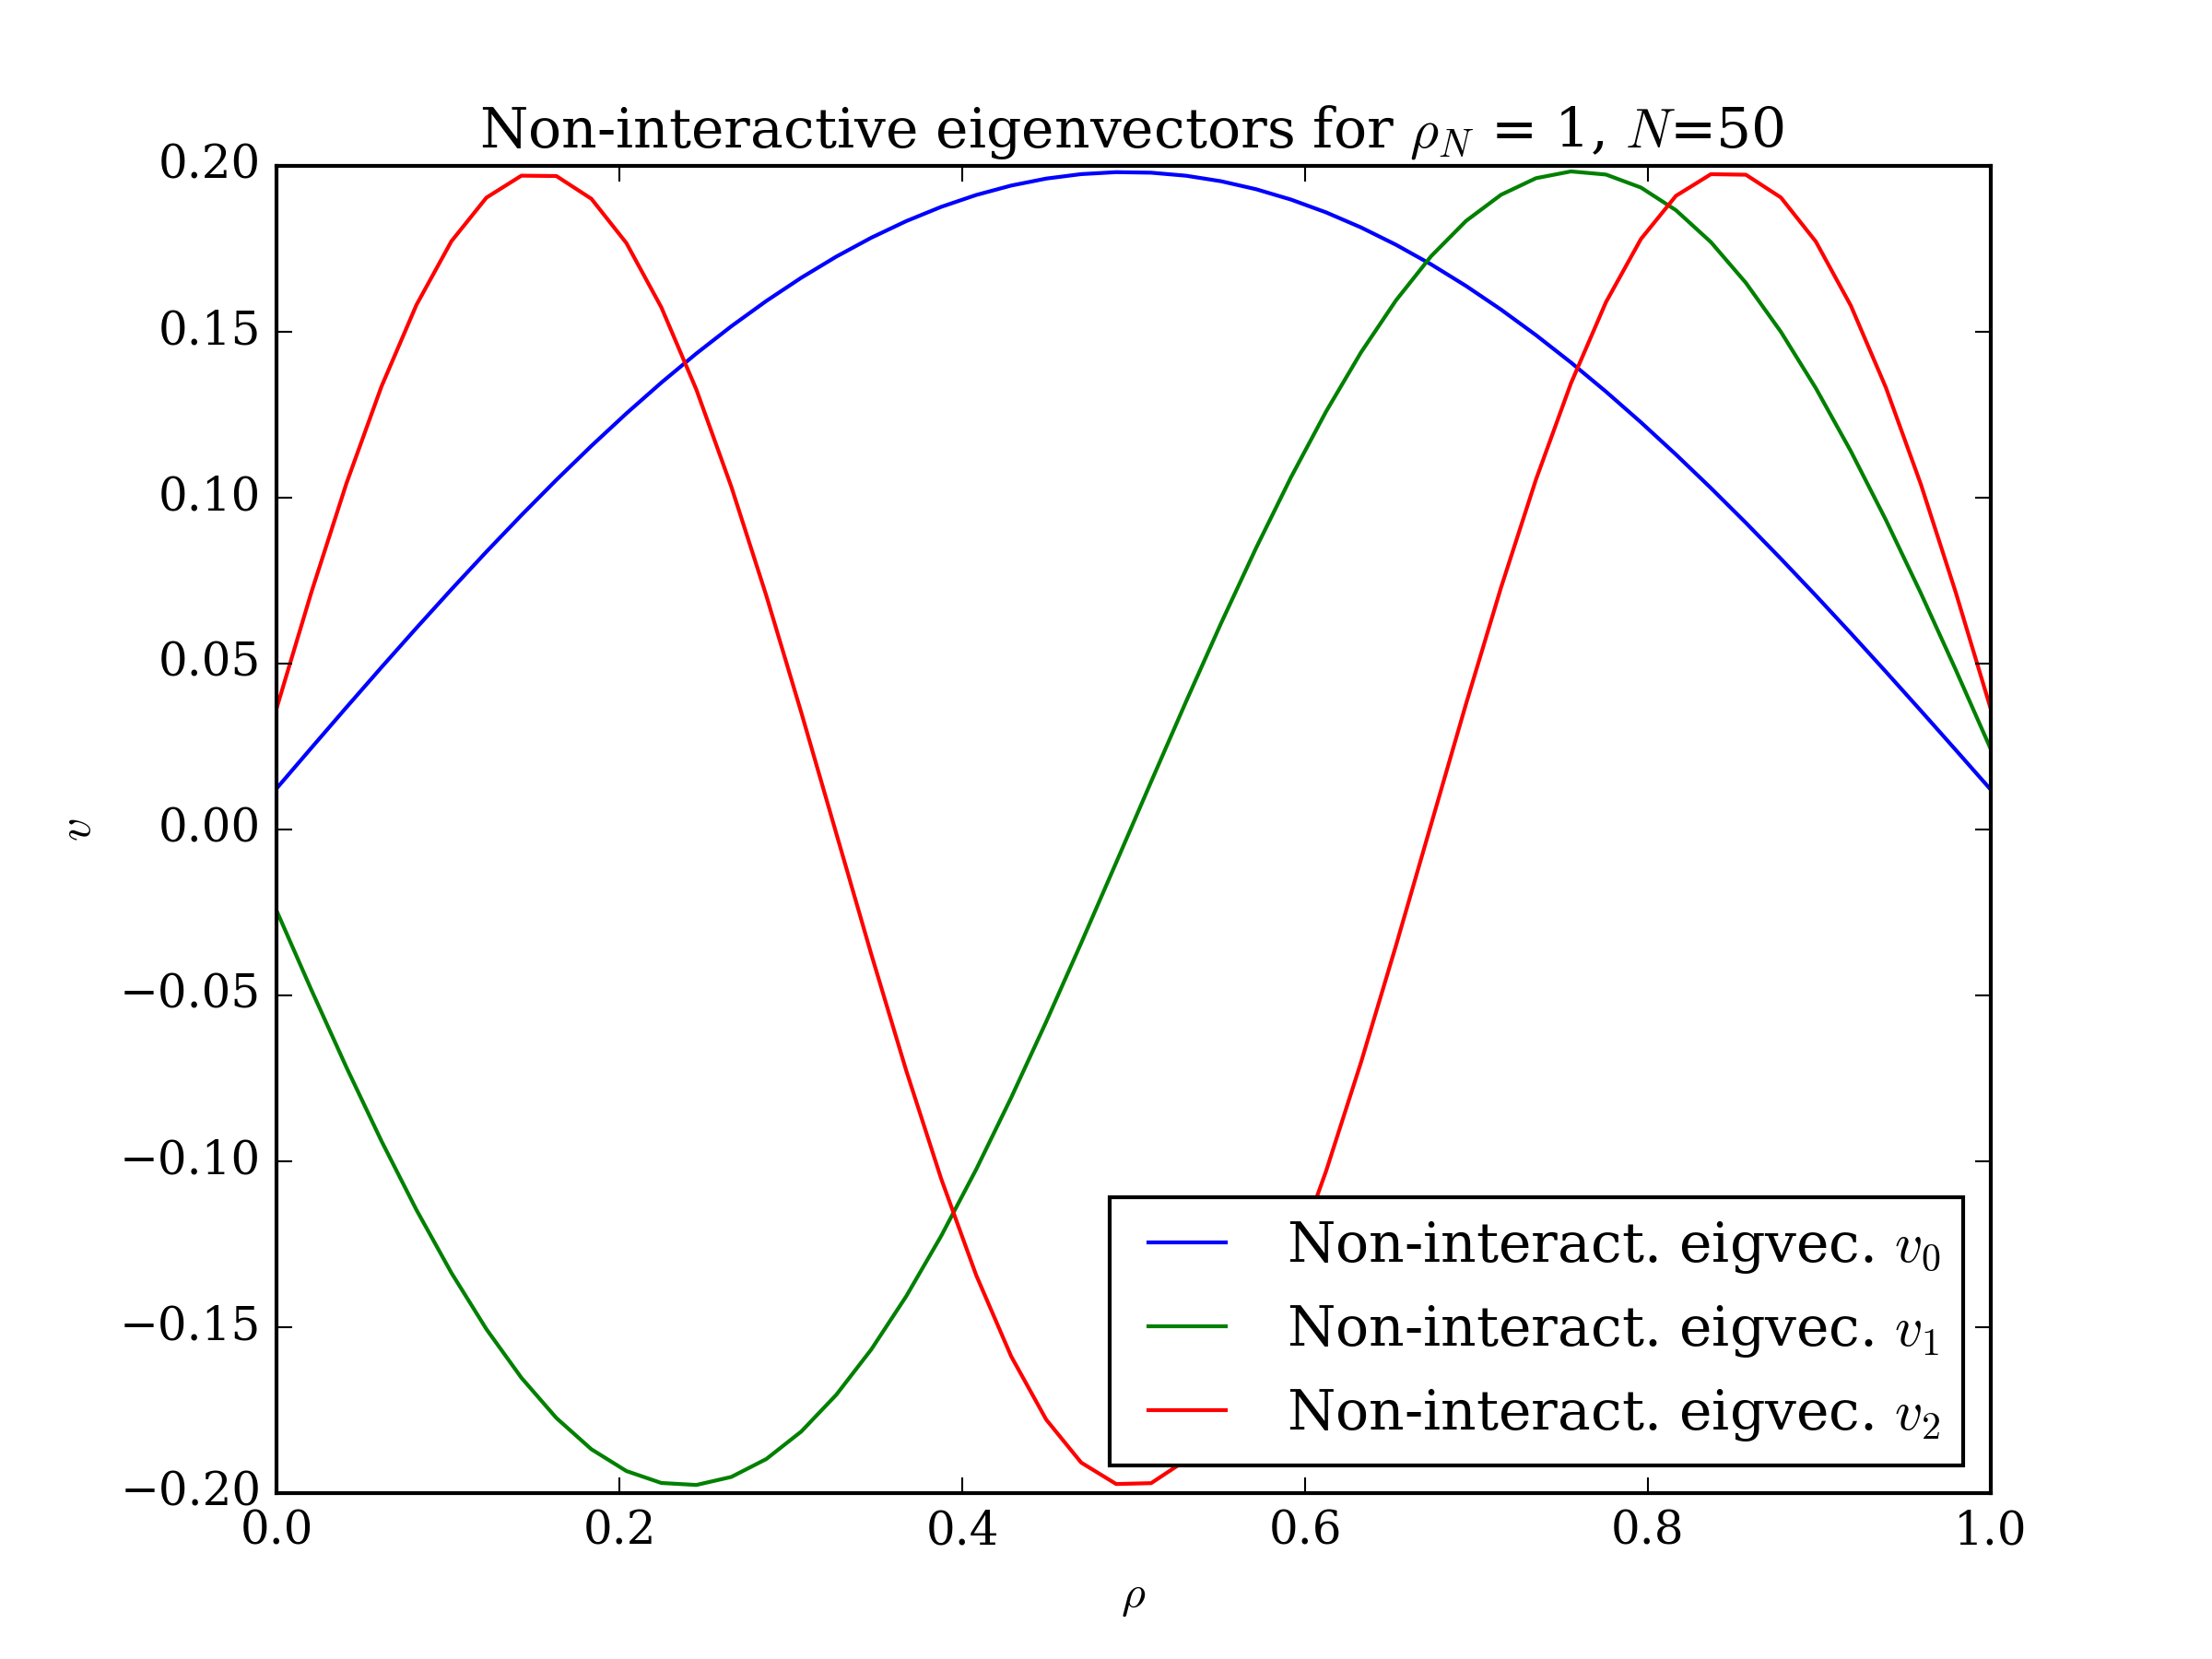
\includegraphics[scale=0.40]{../non_interacting_eigvec_plot_rhoN=1_N=50.png}
        \caption{Non-interactive eigenvectors for $\rho_N = 1$, $N = 50$.}\label{fig:eigvecs-non-interact-1-50}
    \end{subfigure}
    \hfill
    \begin{subfigure}[t]{0.45\textwidth}
        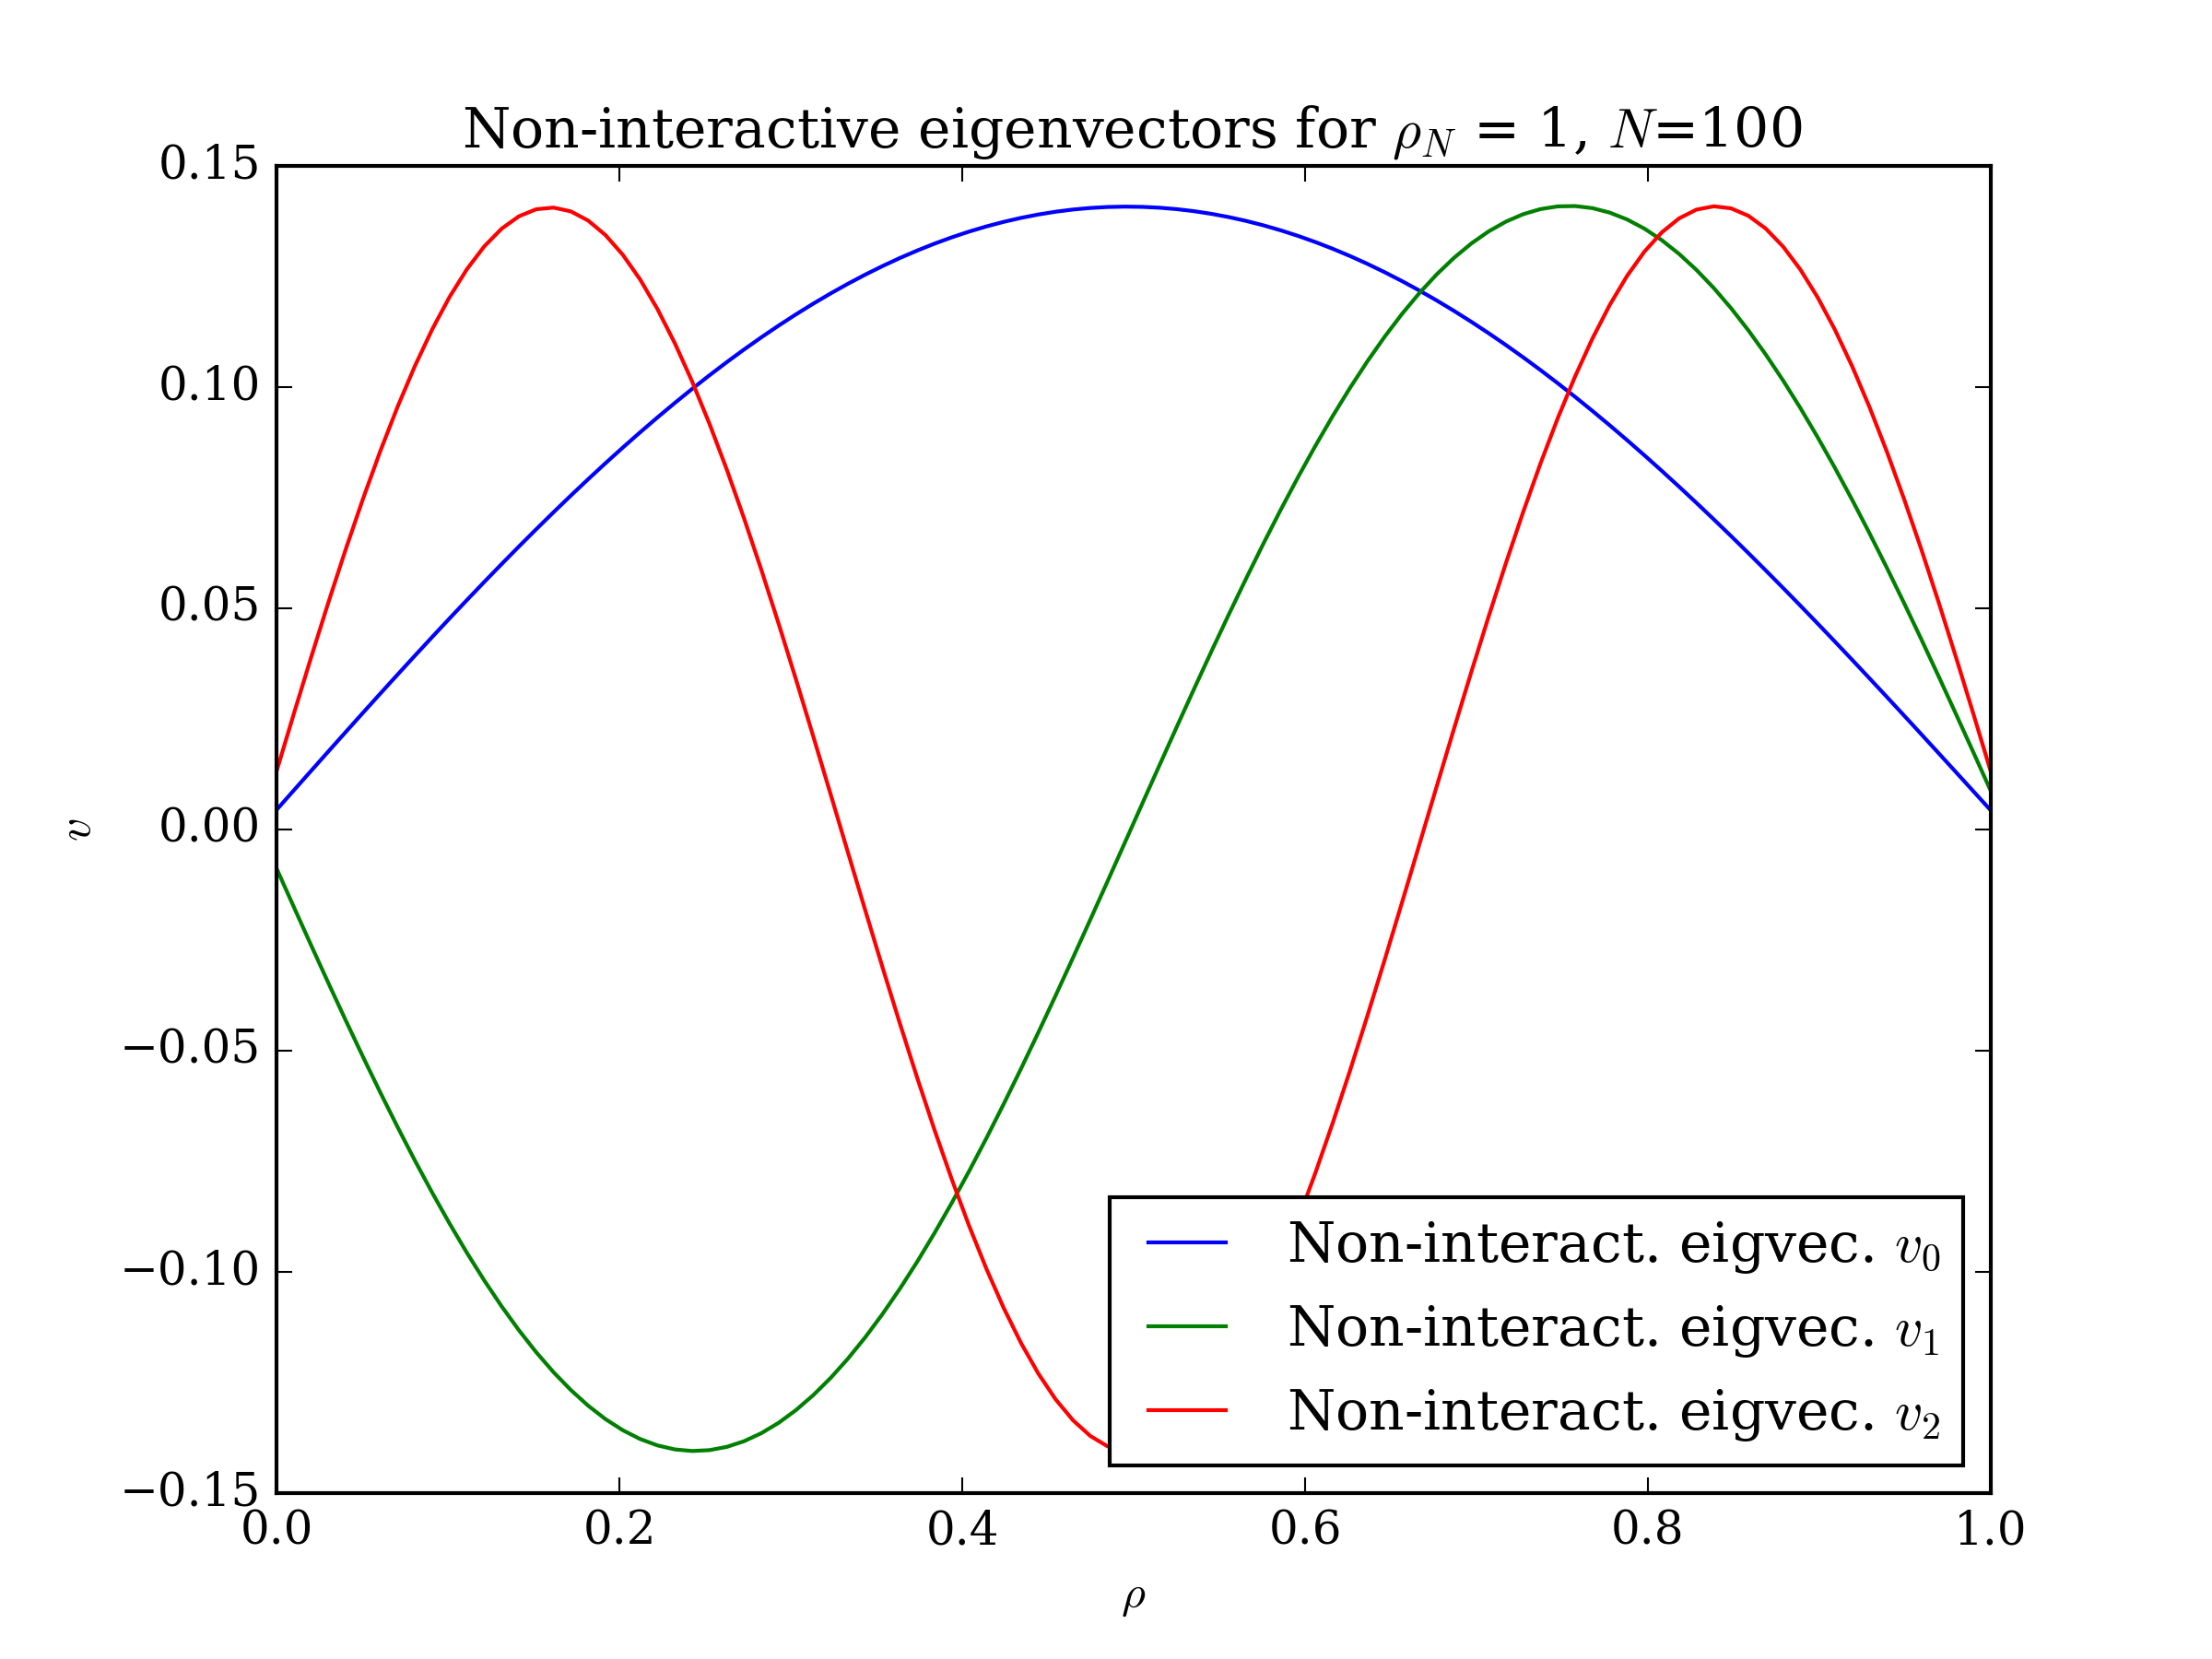
\includegraphics[scale=0.40]{../non_interacting_eigvec_plot_rhoN=1_N=100.png}
        \caption{Non-interactive eigenvectors for $\rho_N = 1$, $N = 100$.}\label{fig:eigvecs-non-interact-1-100}
    \end{subfigure}
    \begin{subfigure}[b]{0.45\textwidth}
        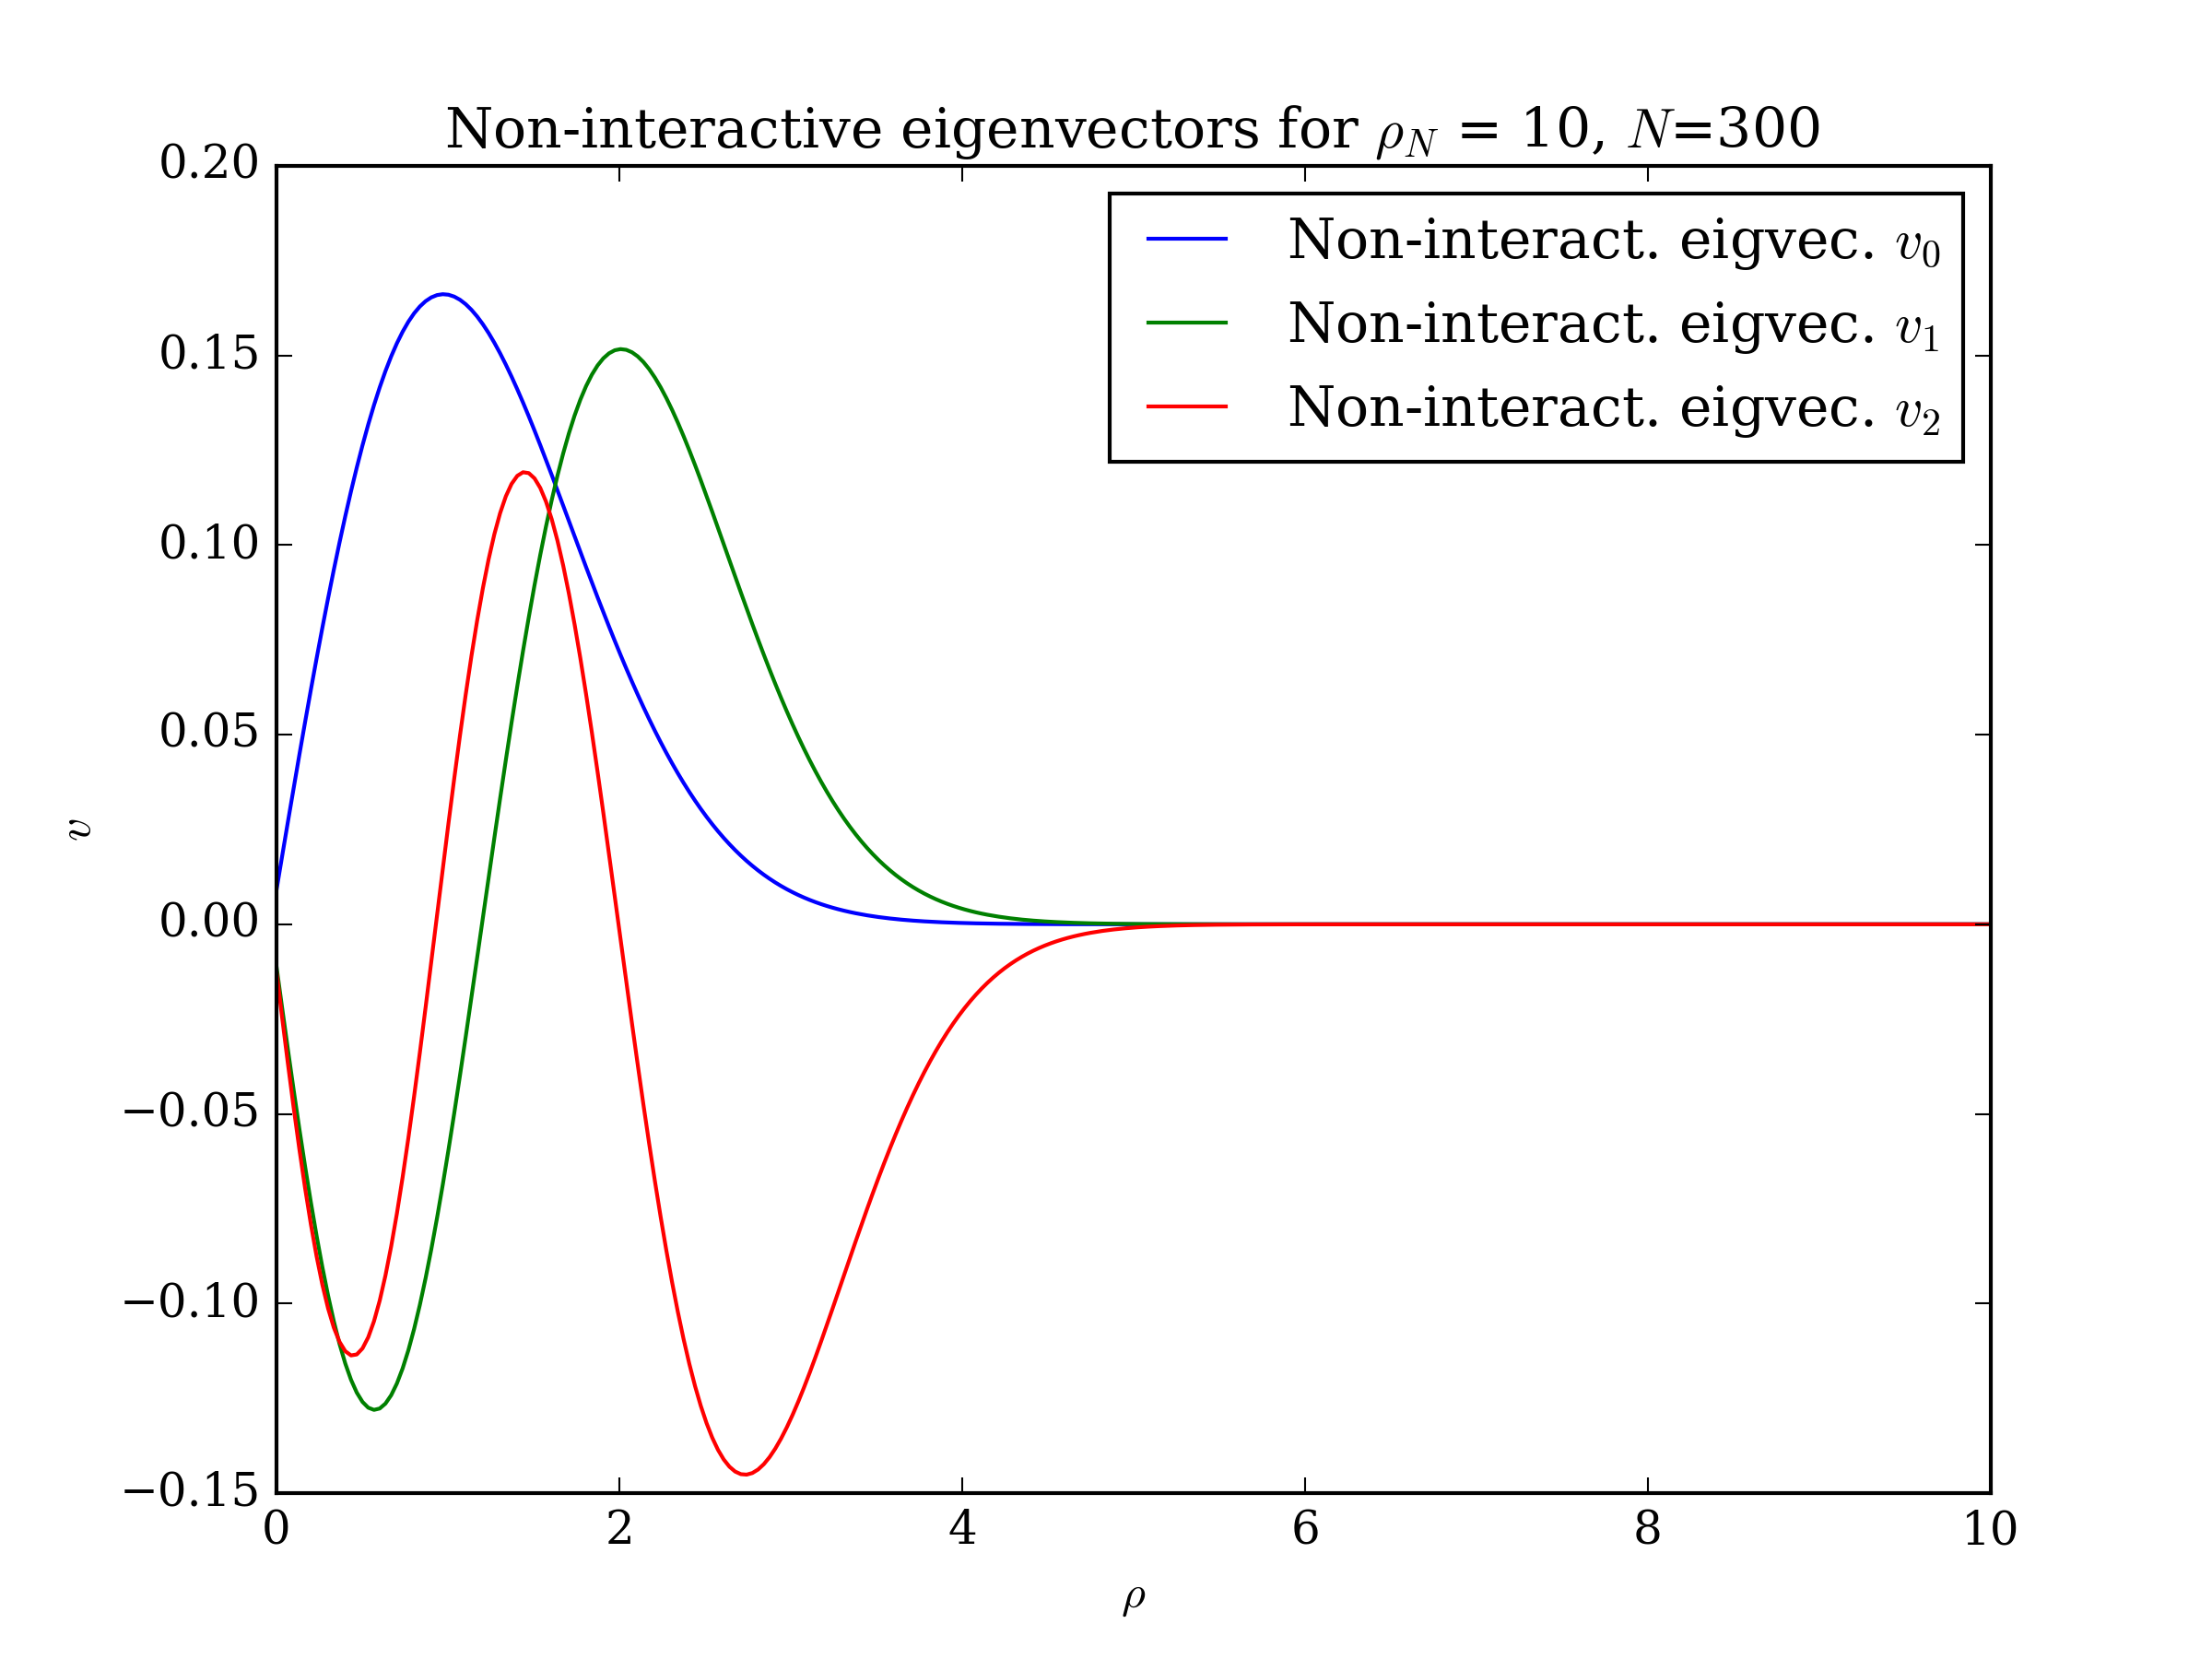
\includegraphics[scale=0.40]{../non_interacting_eigvec_plot_rhoN=10_N=300.png}
        \caption{Non-interactive eigenvectors for $\rho_N = 10$, $N = 300$.}\label{fig:eigvecs-non-interact-10-300}
    \end{subfigure}
    \hfill
    \begin{subfigure}[b]{0.45\textwidth}
        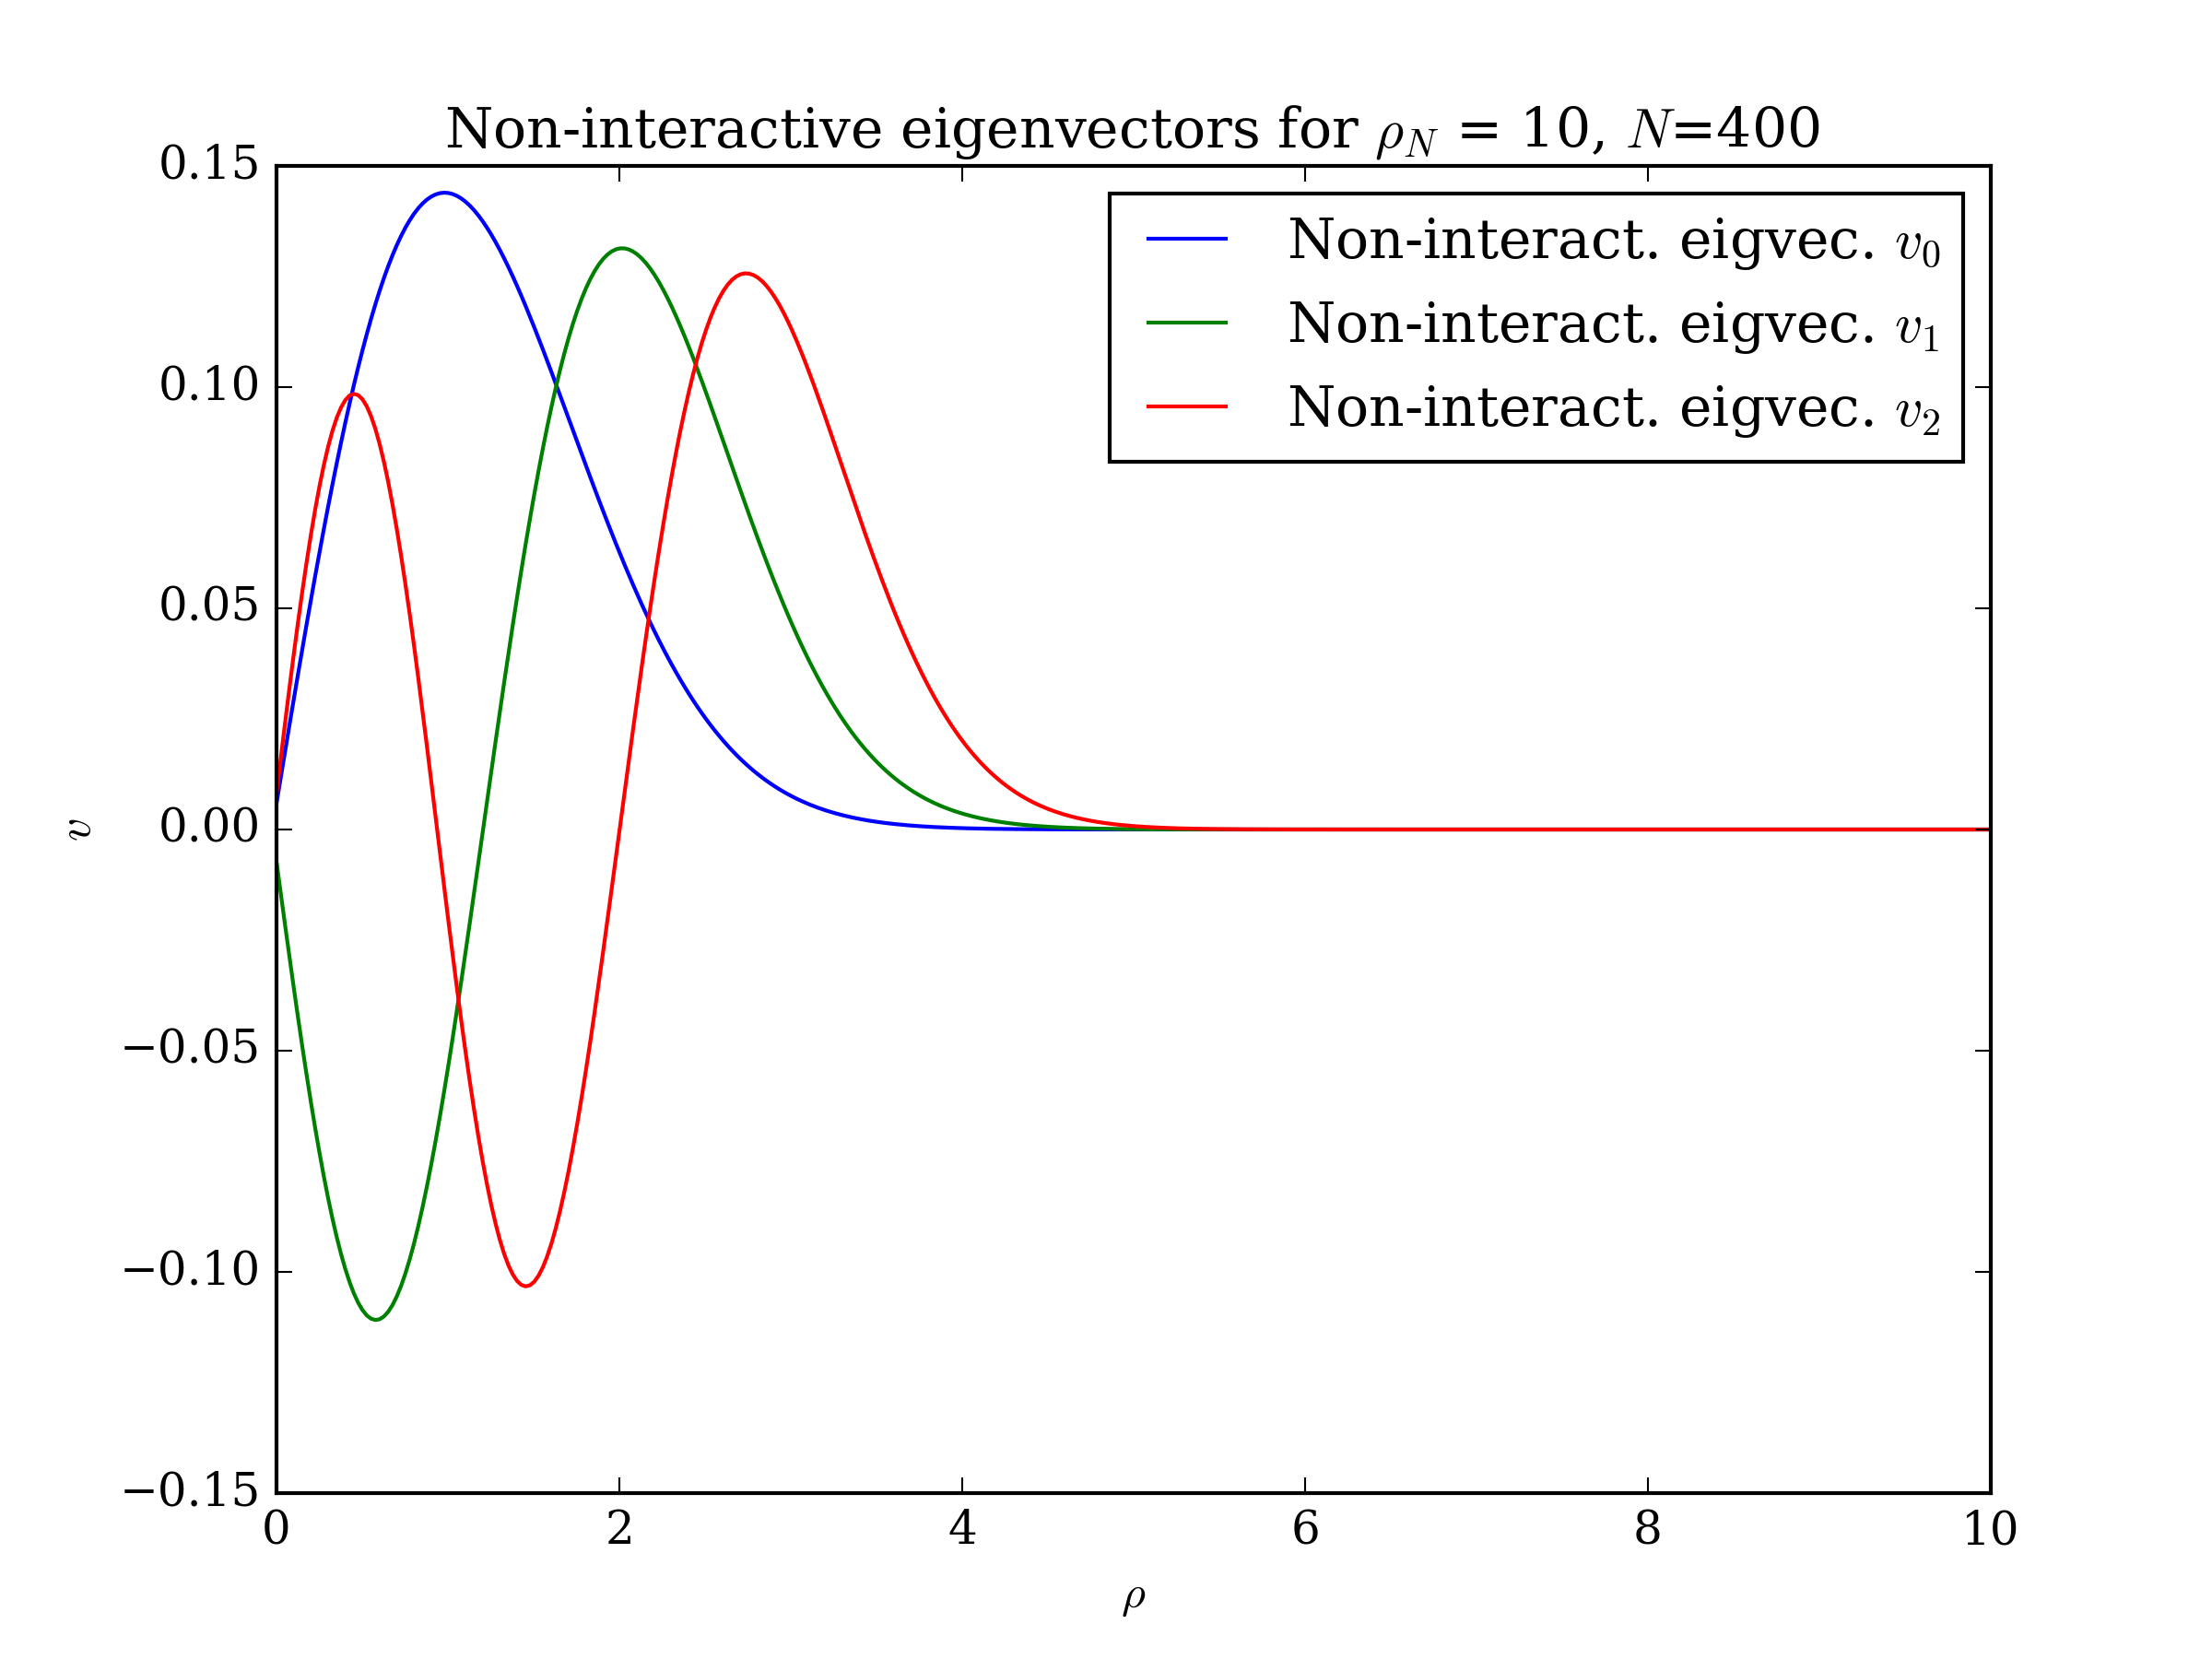
\includegraphics[scale=0.40]{../non_interacting_eigvec_plot_rhoN=10_N=400.png}
        \caption{Non-interactive eigenvectors for $\rho_N = 10$, $N = 400$.}\label{fig:eigvecs-non-interact-10-400}
    \end{subfigure}
\begin{subfigure}[t]{0.45\textwidth}
        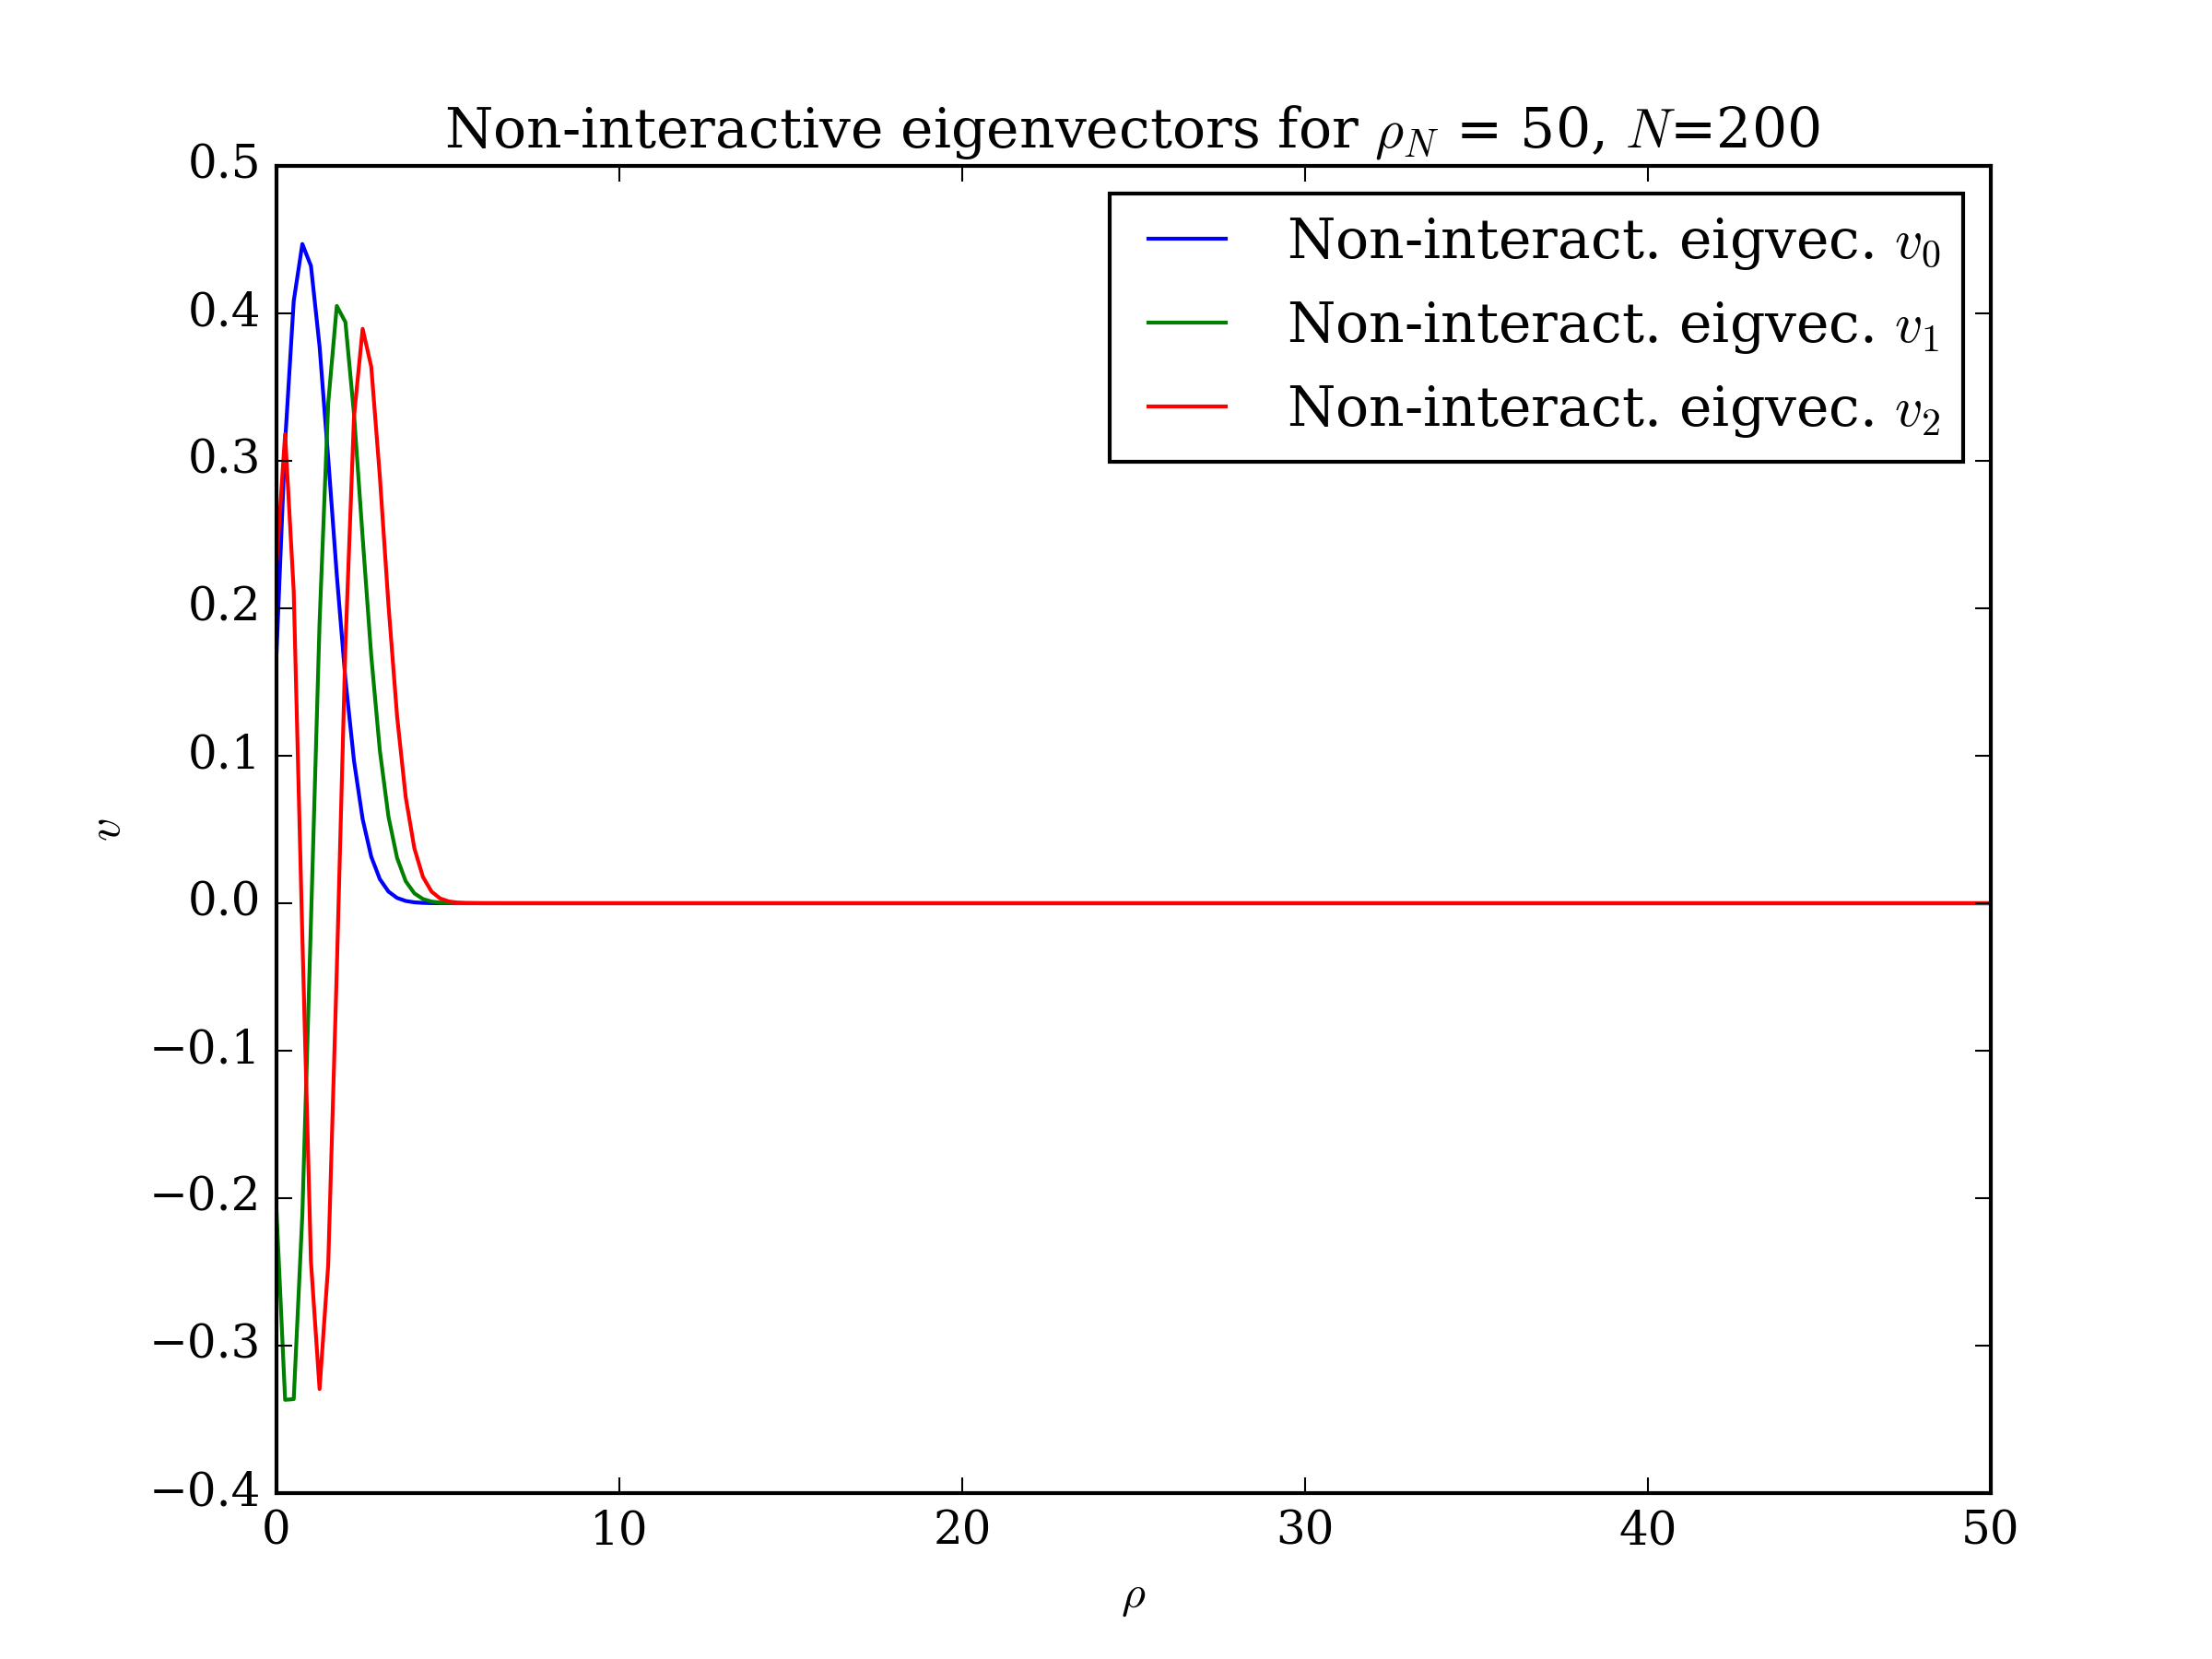
\includegraphics[scale=0.40]{../non_interacting_eigvec_plot_rhoN=50_N=200.png}
        \caption{Non-interactive eigenvectors for $\rho_N = 50$, $N = 200$.}\label{fig:eigvecs-non-interact-50-200}
\end{subfigure}
    \caption{A set of ground state for interactions at different values of $\omega_r$.}\label{fig:eigvecs-non-interact}
\end{figure}
For the interacting cases of the numerical eigenvector extraction, these plots were yielded by use of the scripts.
\begin{figure}[H]
\center
    \begin{subfigure}[t]{0.45\textwidth}
        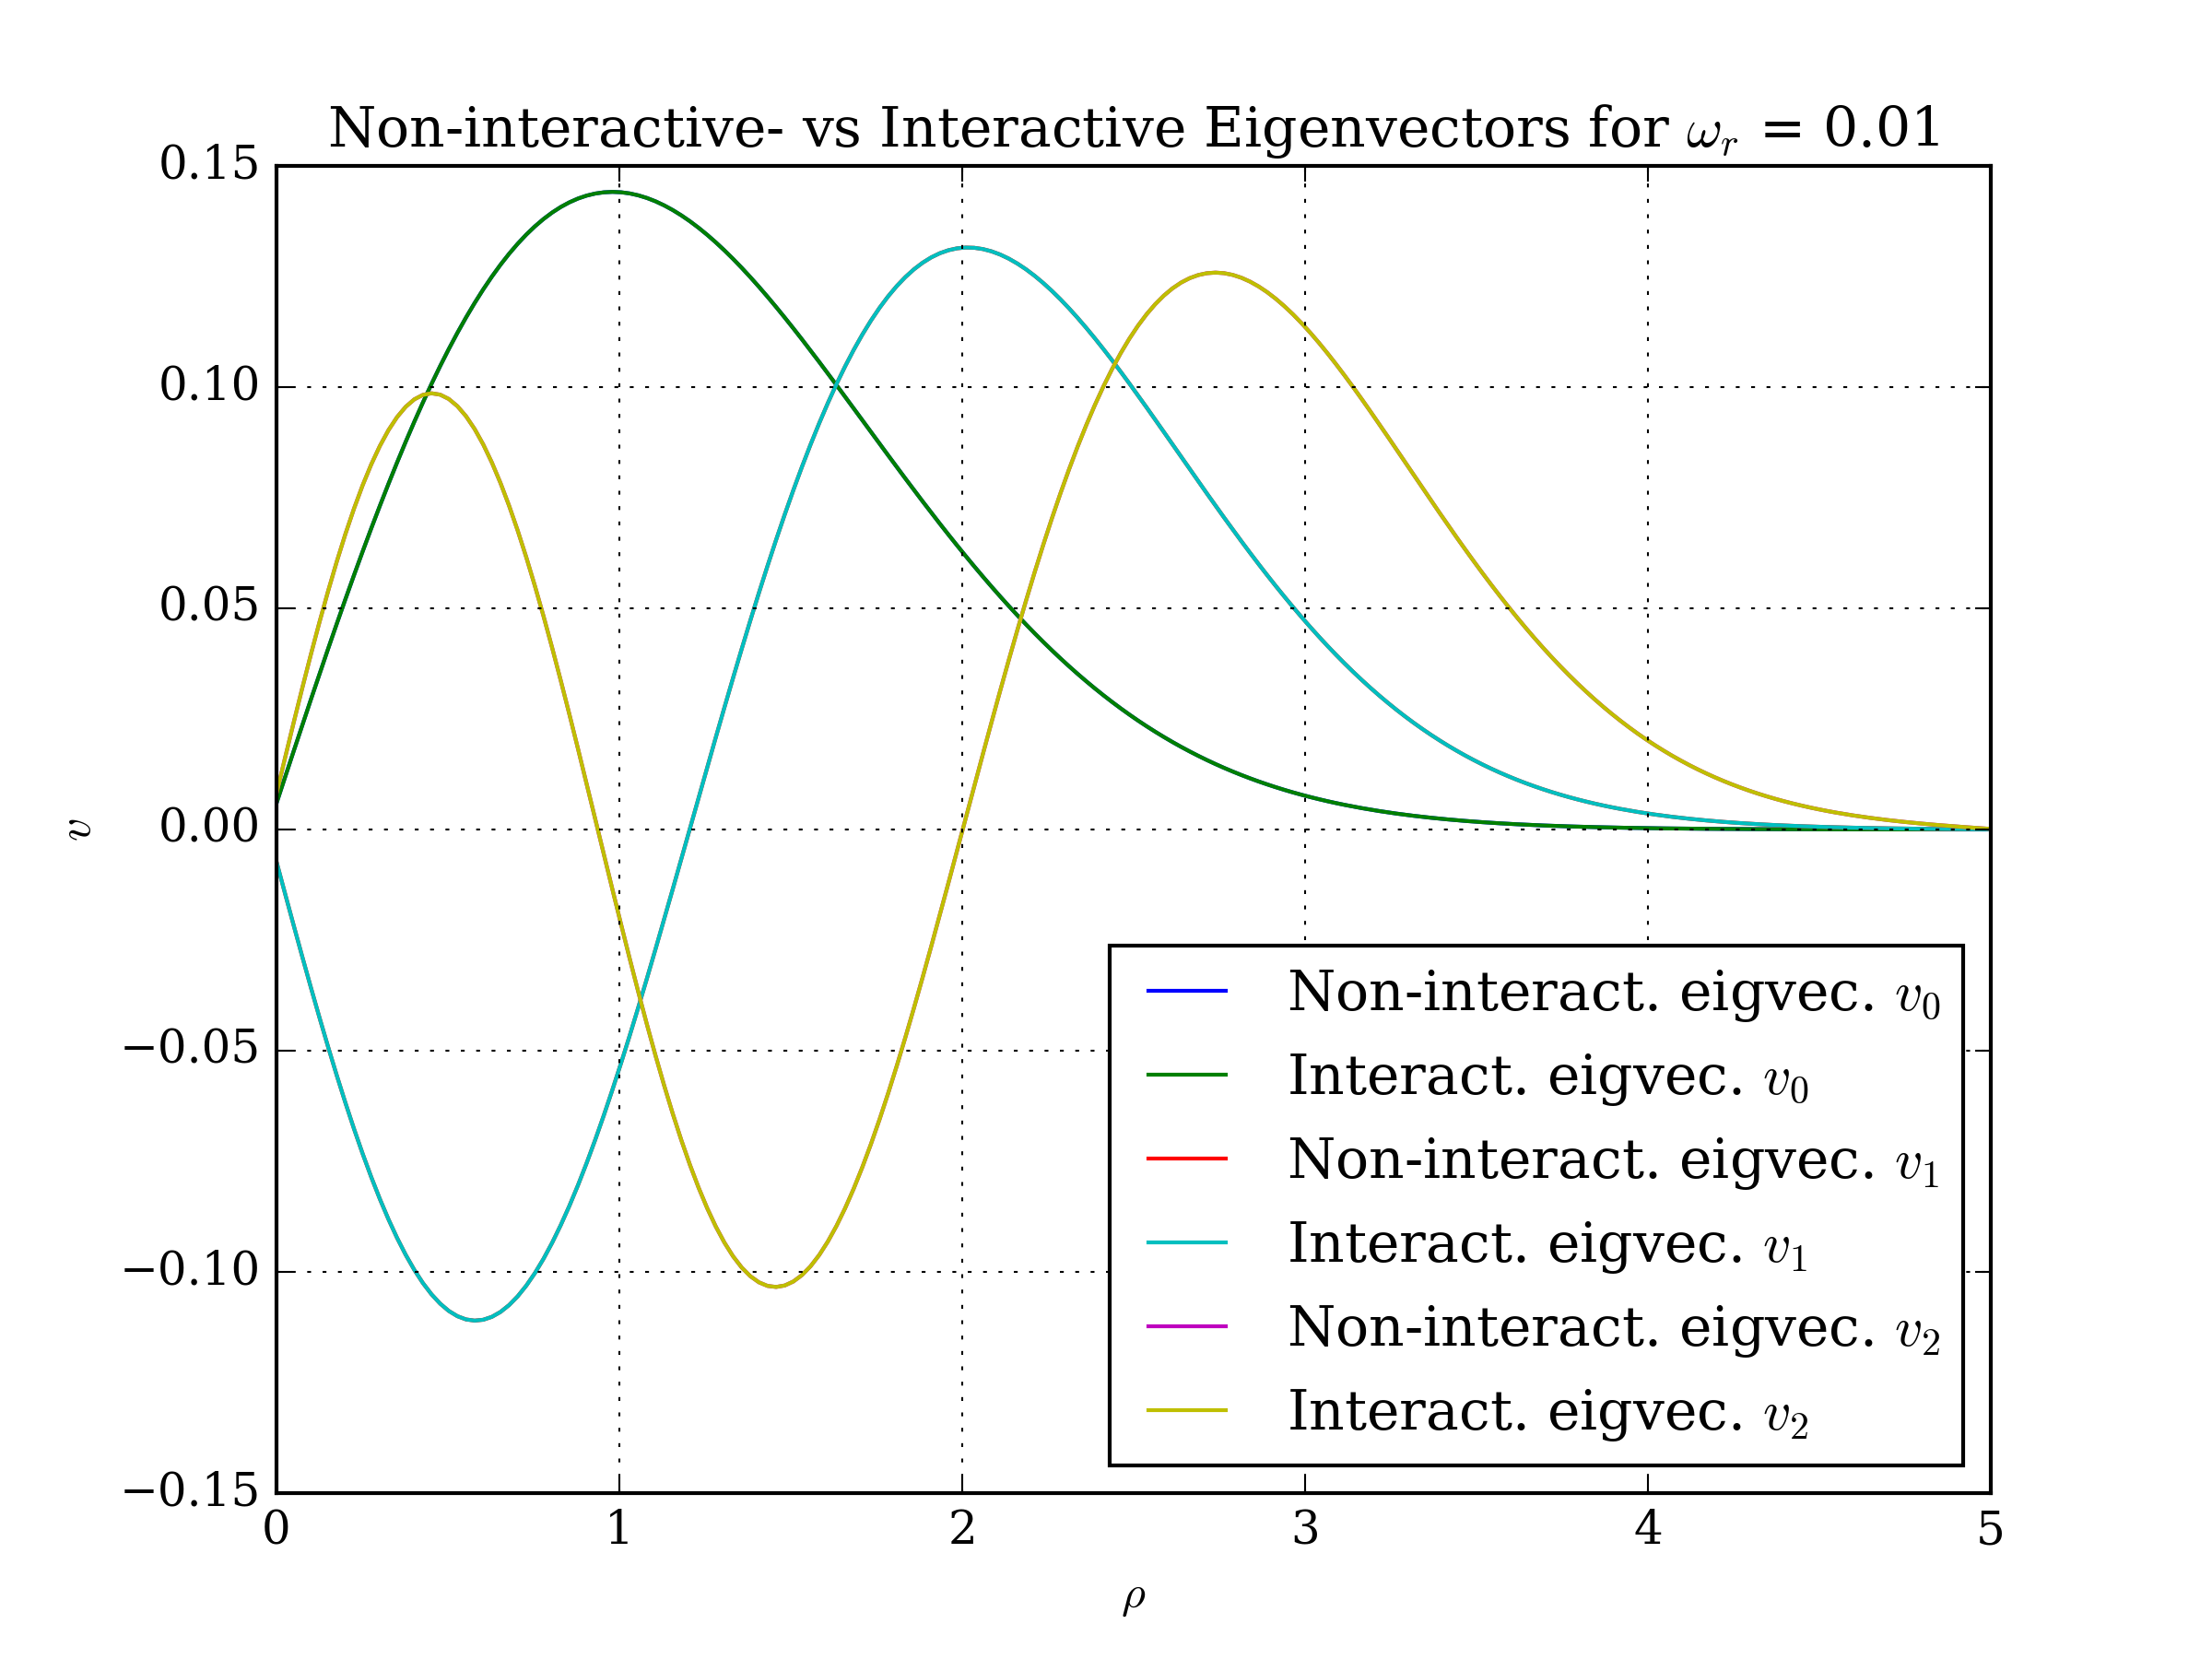
\includegraphics[scale=0.40]{../interacting_eigvecs_at_omega=10.png}
        \caption{Ground state eigenvectors for both interacting and non-interacting case, at $\omega_r = 0.01$.}\label{fig:eigvecs-interact10}
    \end{subfigure}
    \hfill
    \begin{subfigure}[t]{0.45\textwidth}
        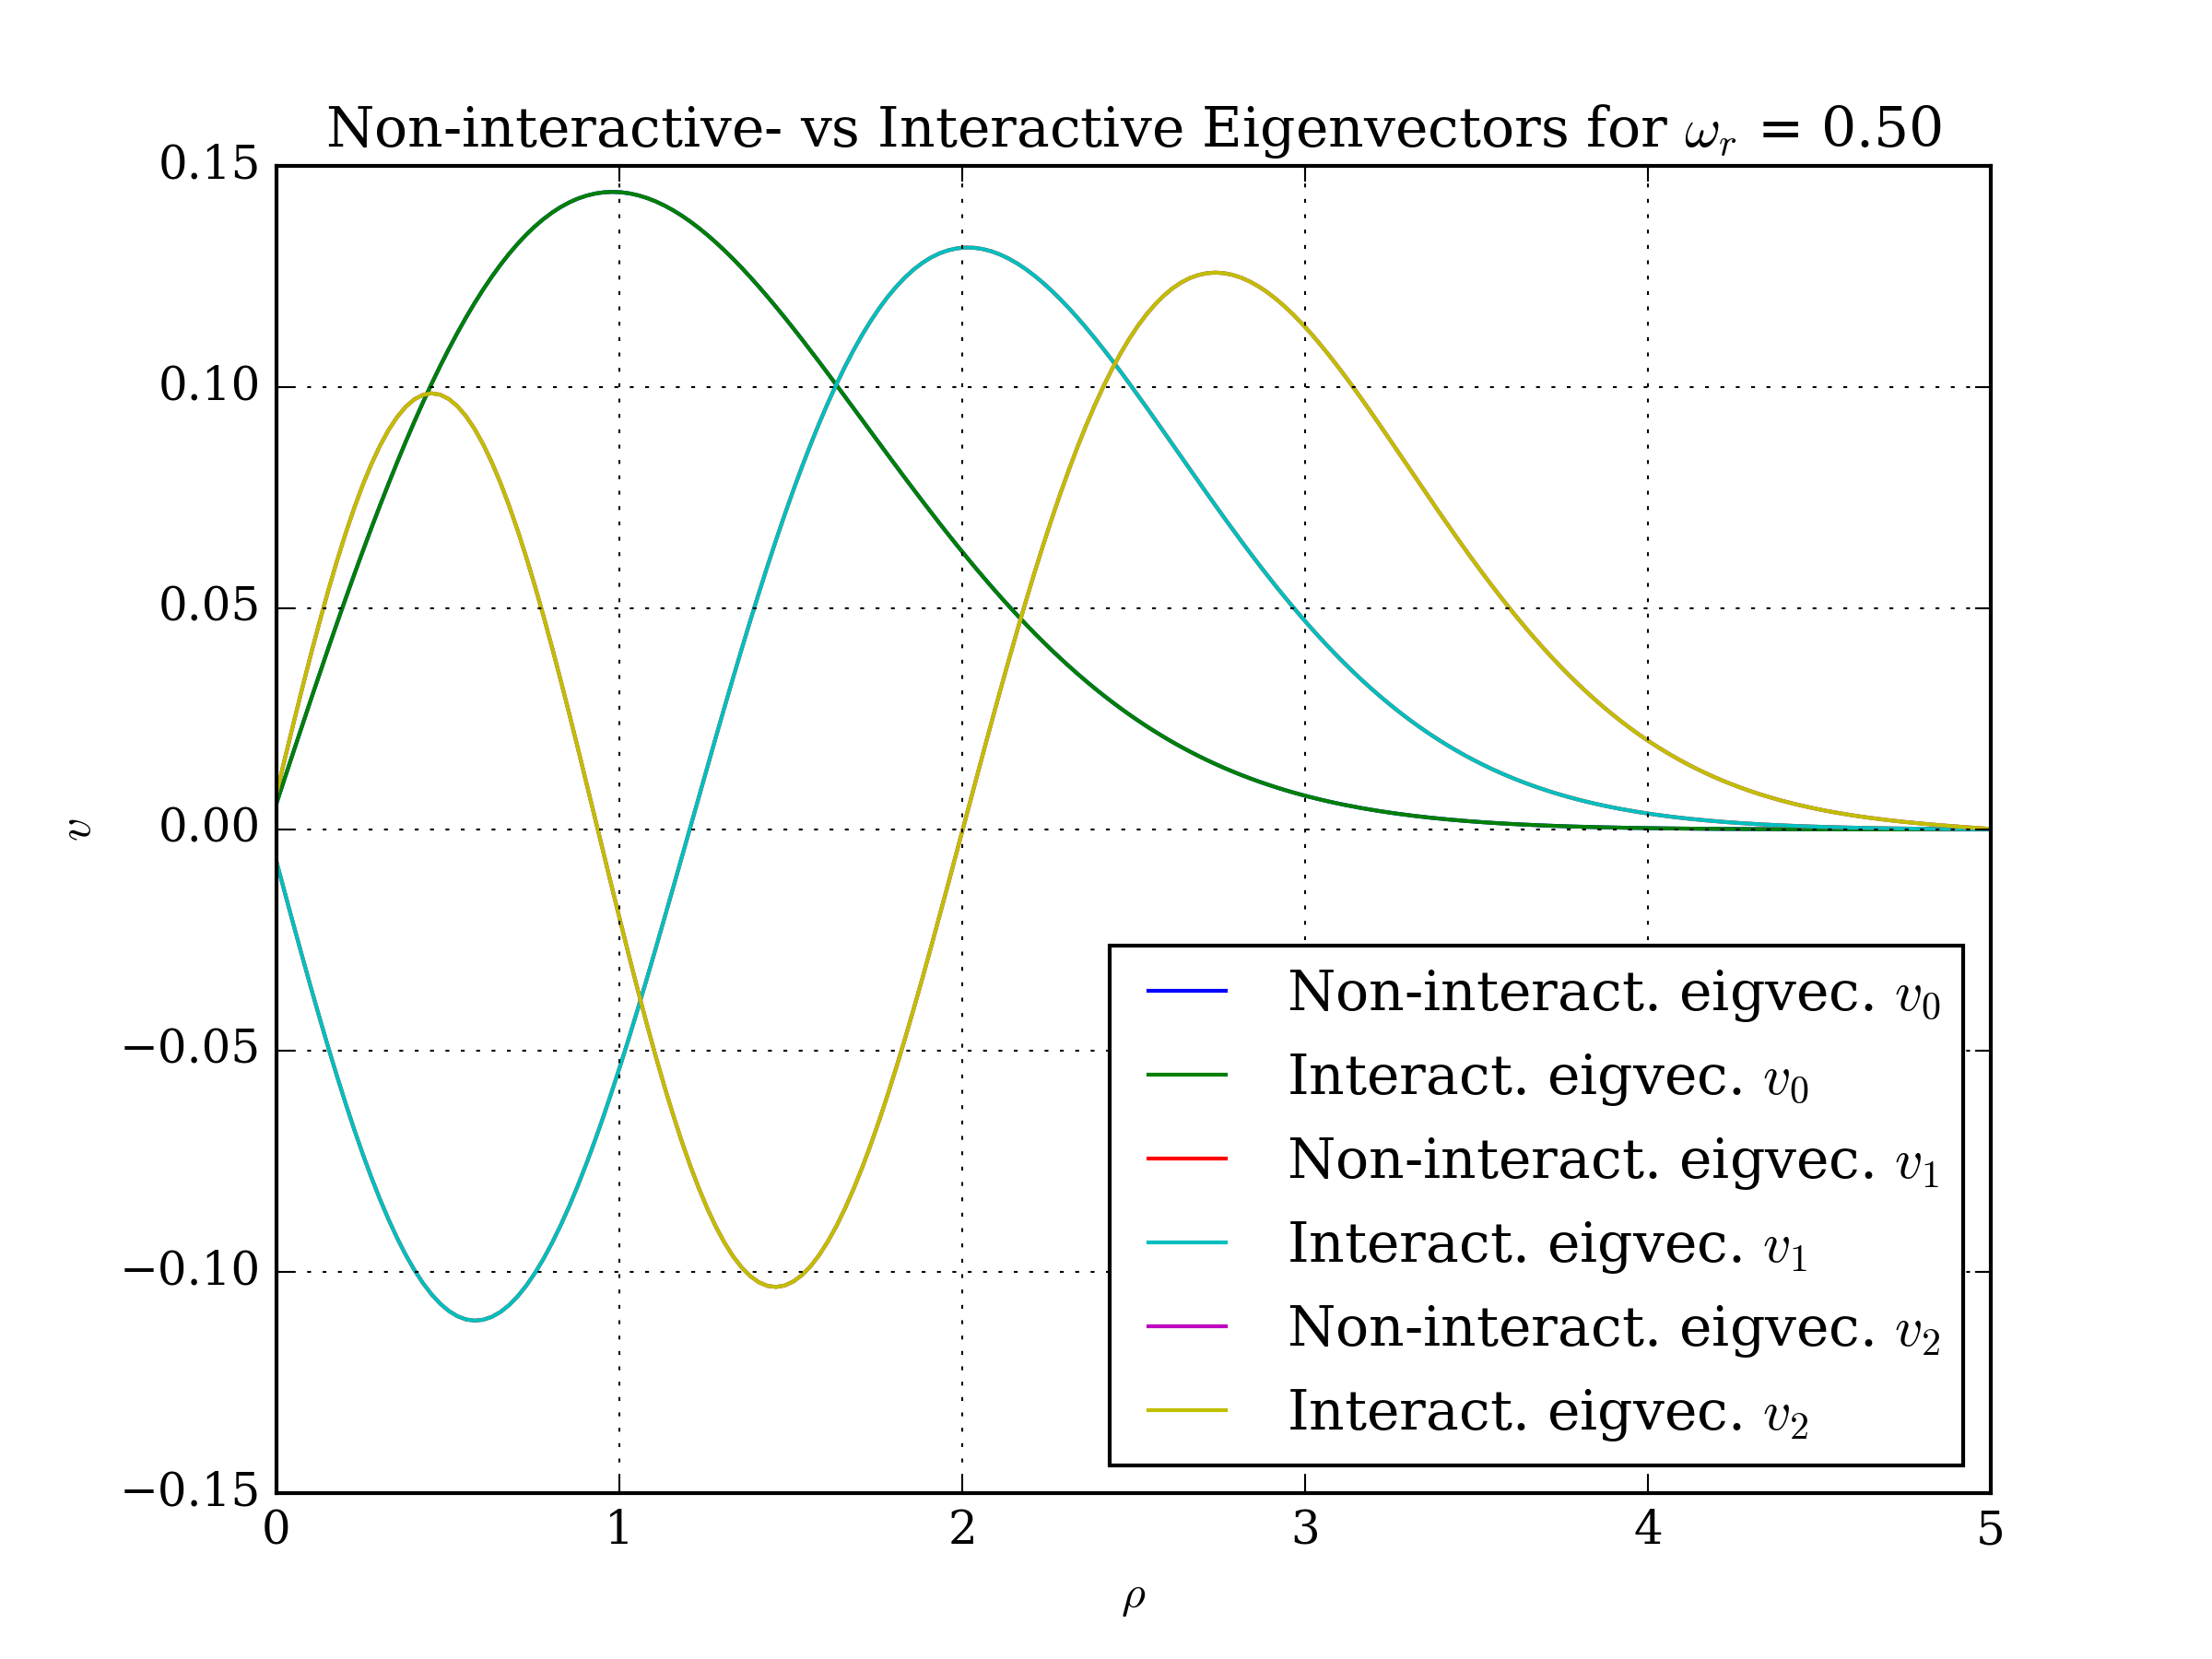
\includegraphics[scale=0.40]{../interacting_eigvecs_at_omega=500.png}
        \caption{Ground state eigenvectors for both interacting and non-interacting case, at $\omega_r = 0.5$.}\label{fig:eigvecs-interact500}
    \end{subfigure}
    \begin{subfigure}[b]{0.45\textwidth}
        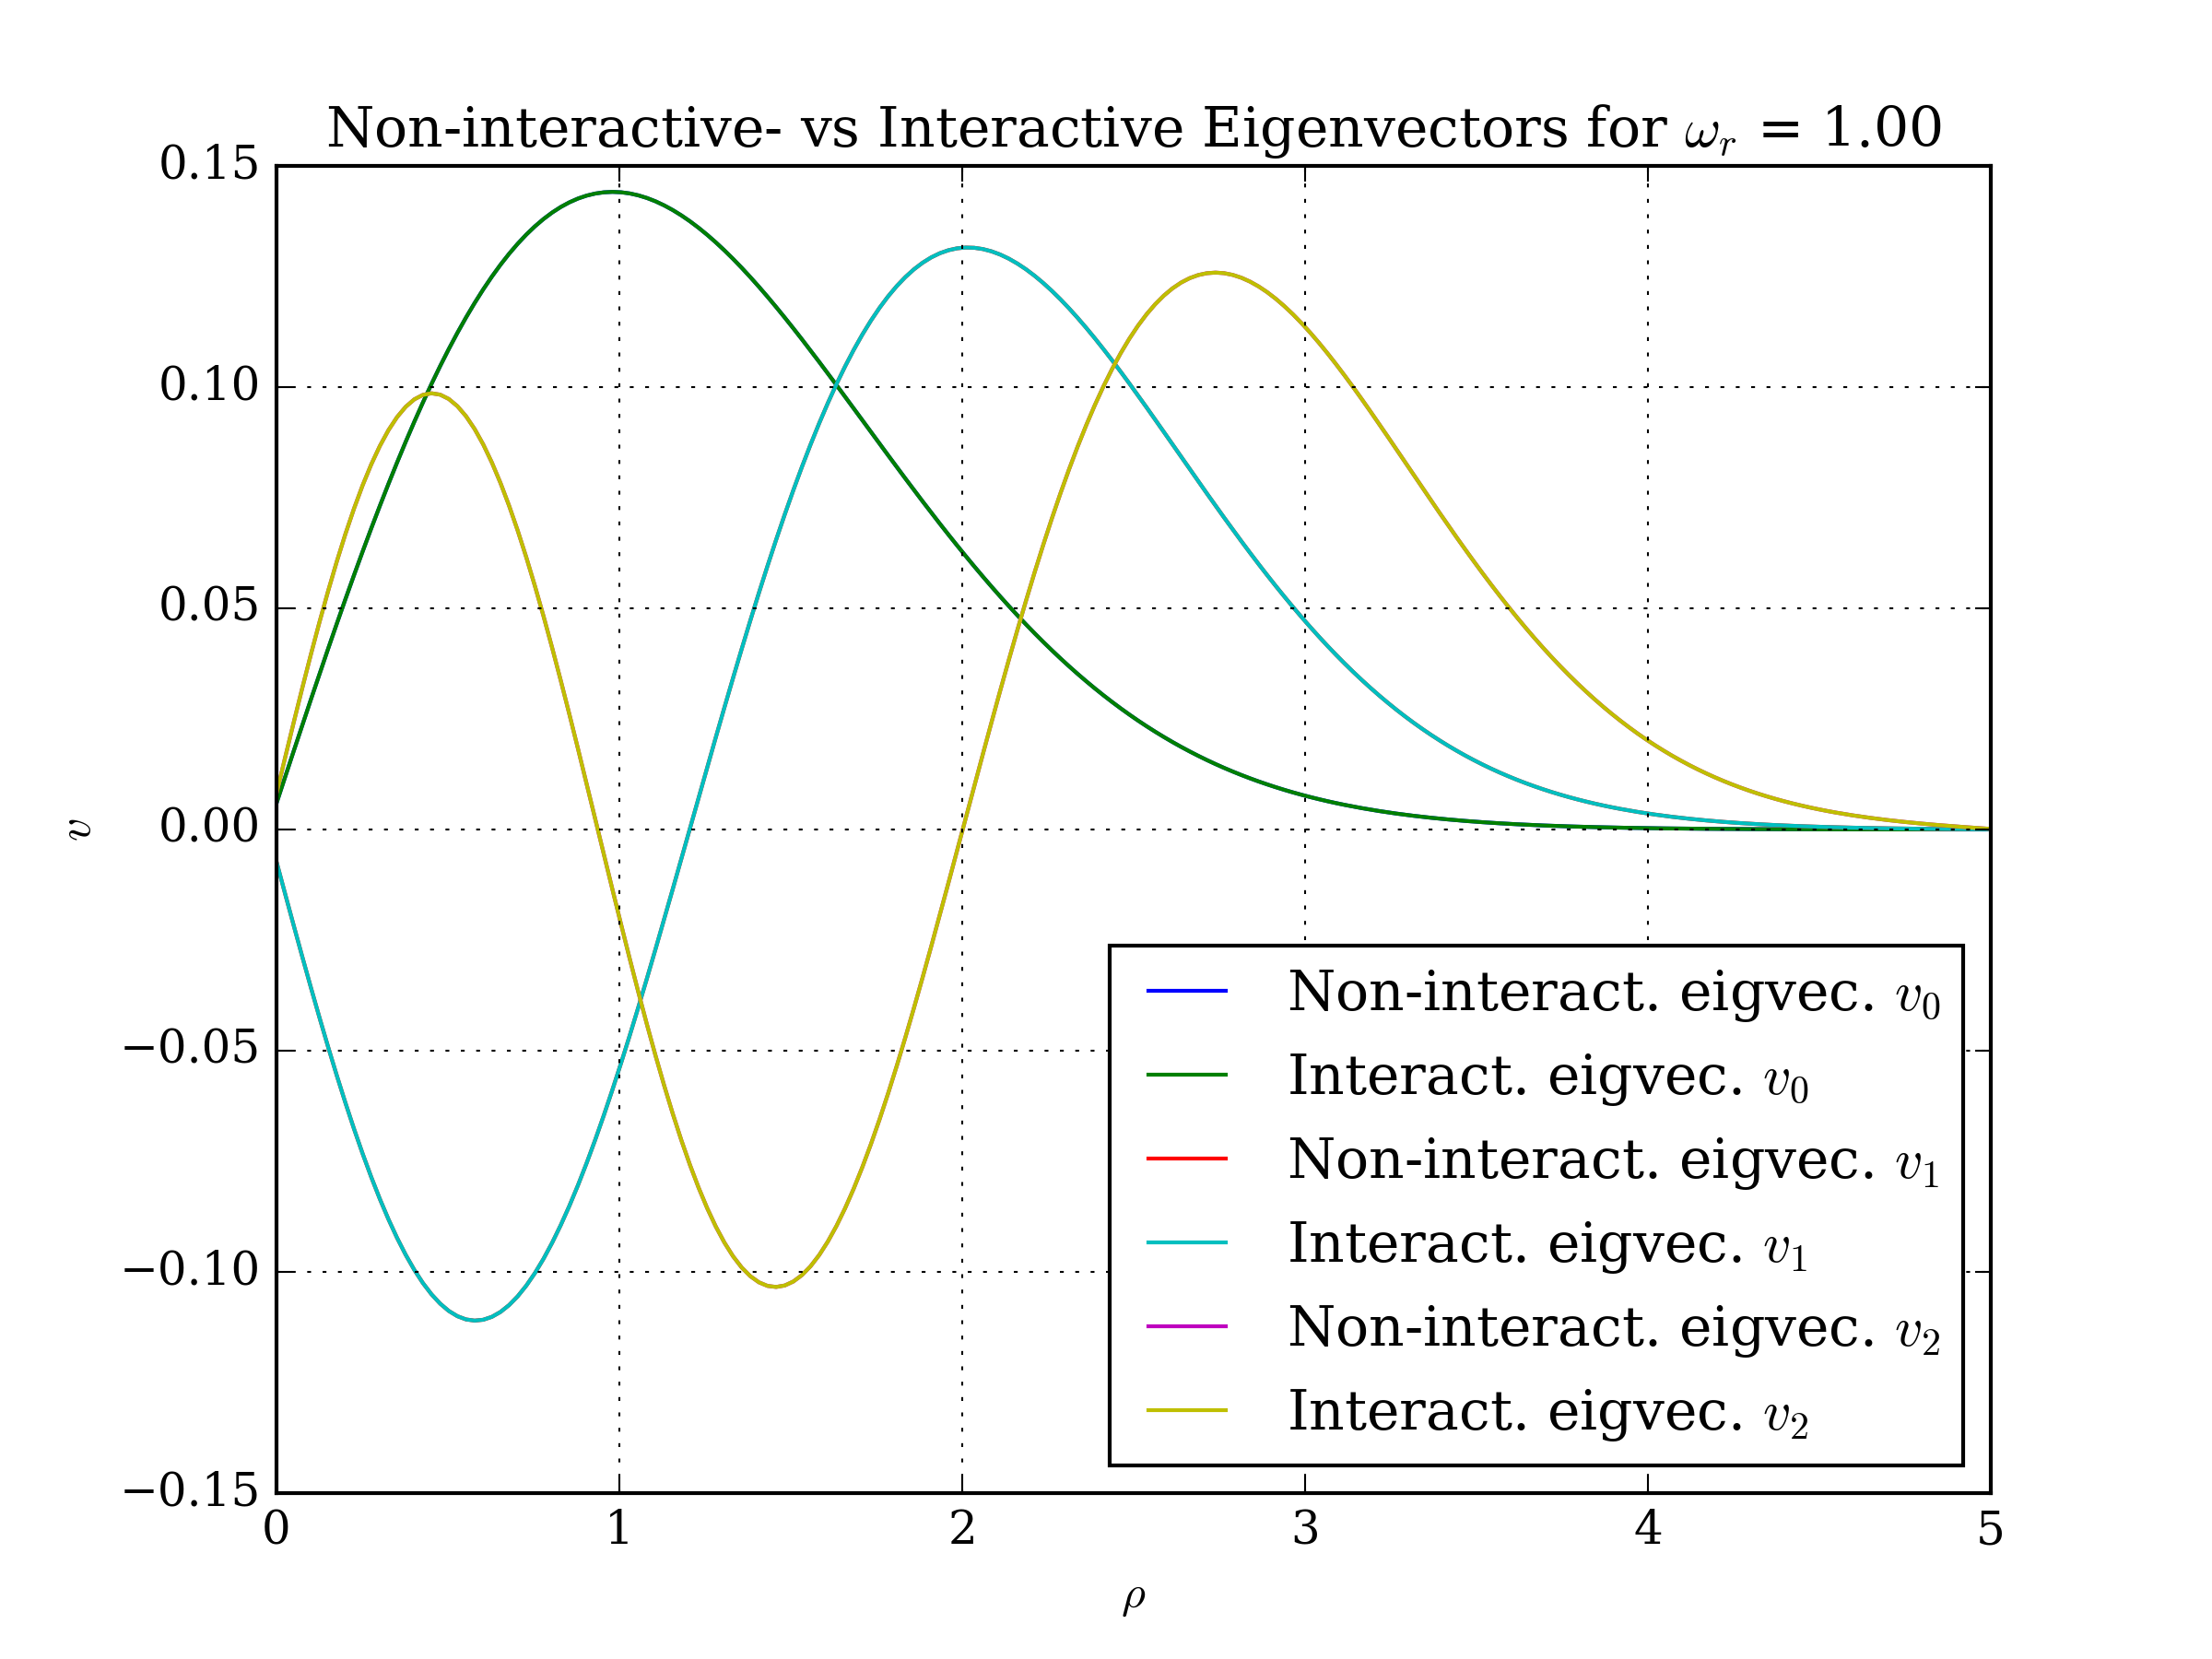
\includegraphics[scale=0.40]{../interacting_eigvecs_at_omega=1000.png}
        \caption{Ground state eigenvectors for both interacting and non-interacting case, at $\omega_r = 1$.}\label{fig:eigvecs-interact1000}
    \end{subfigure}
    \hfill
    \begin{subfigure}[b]{0.45\textwidth}
        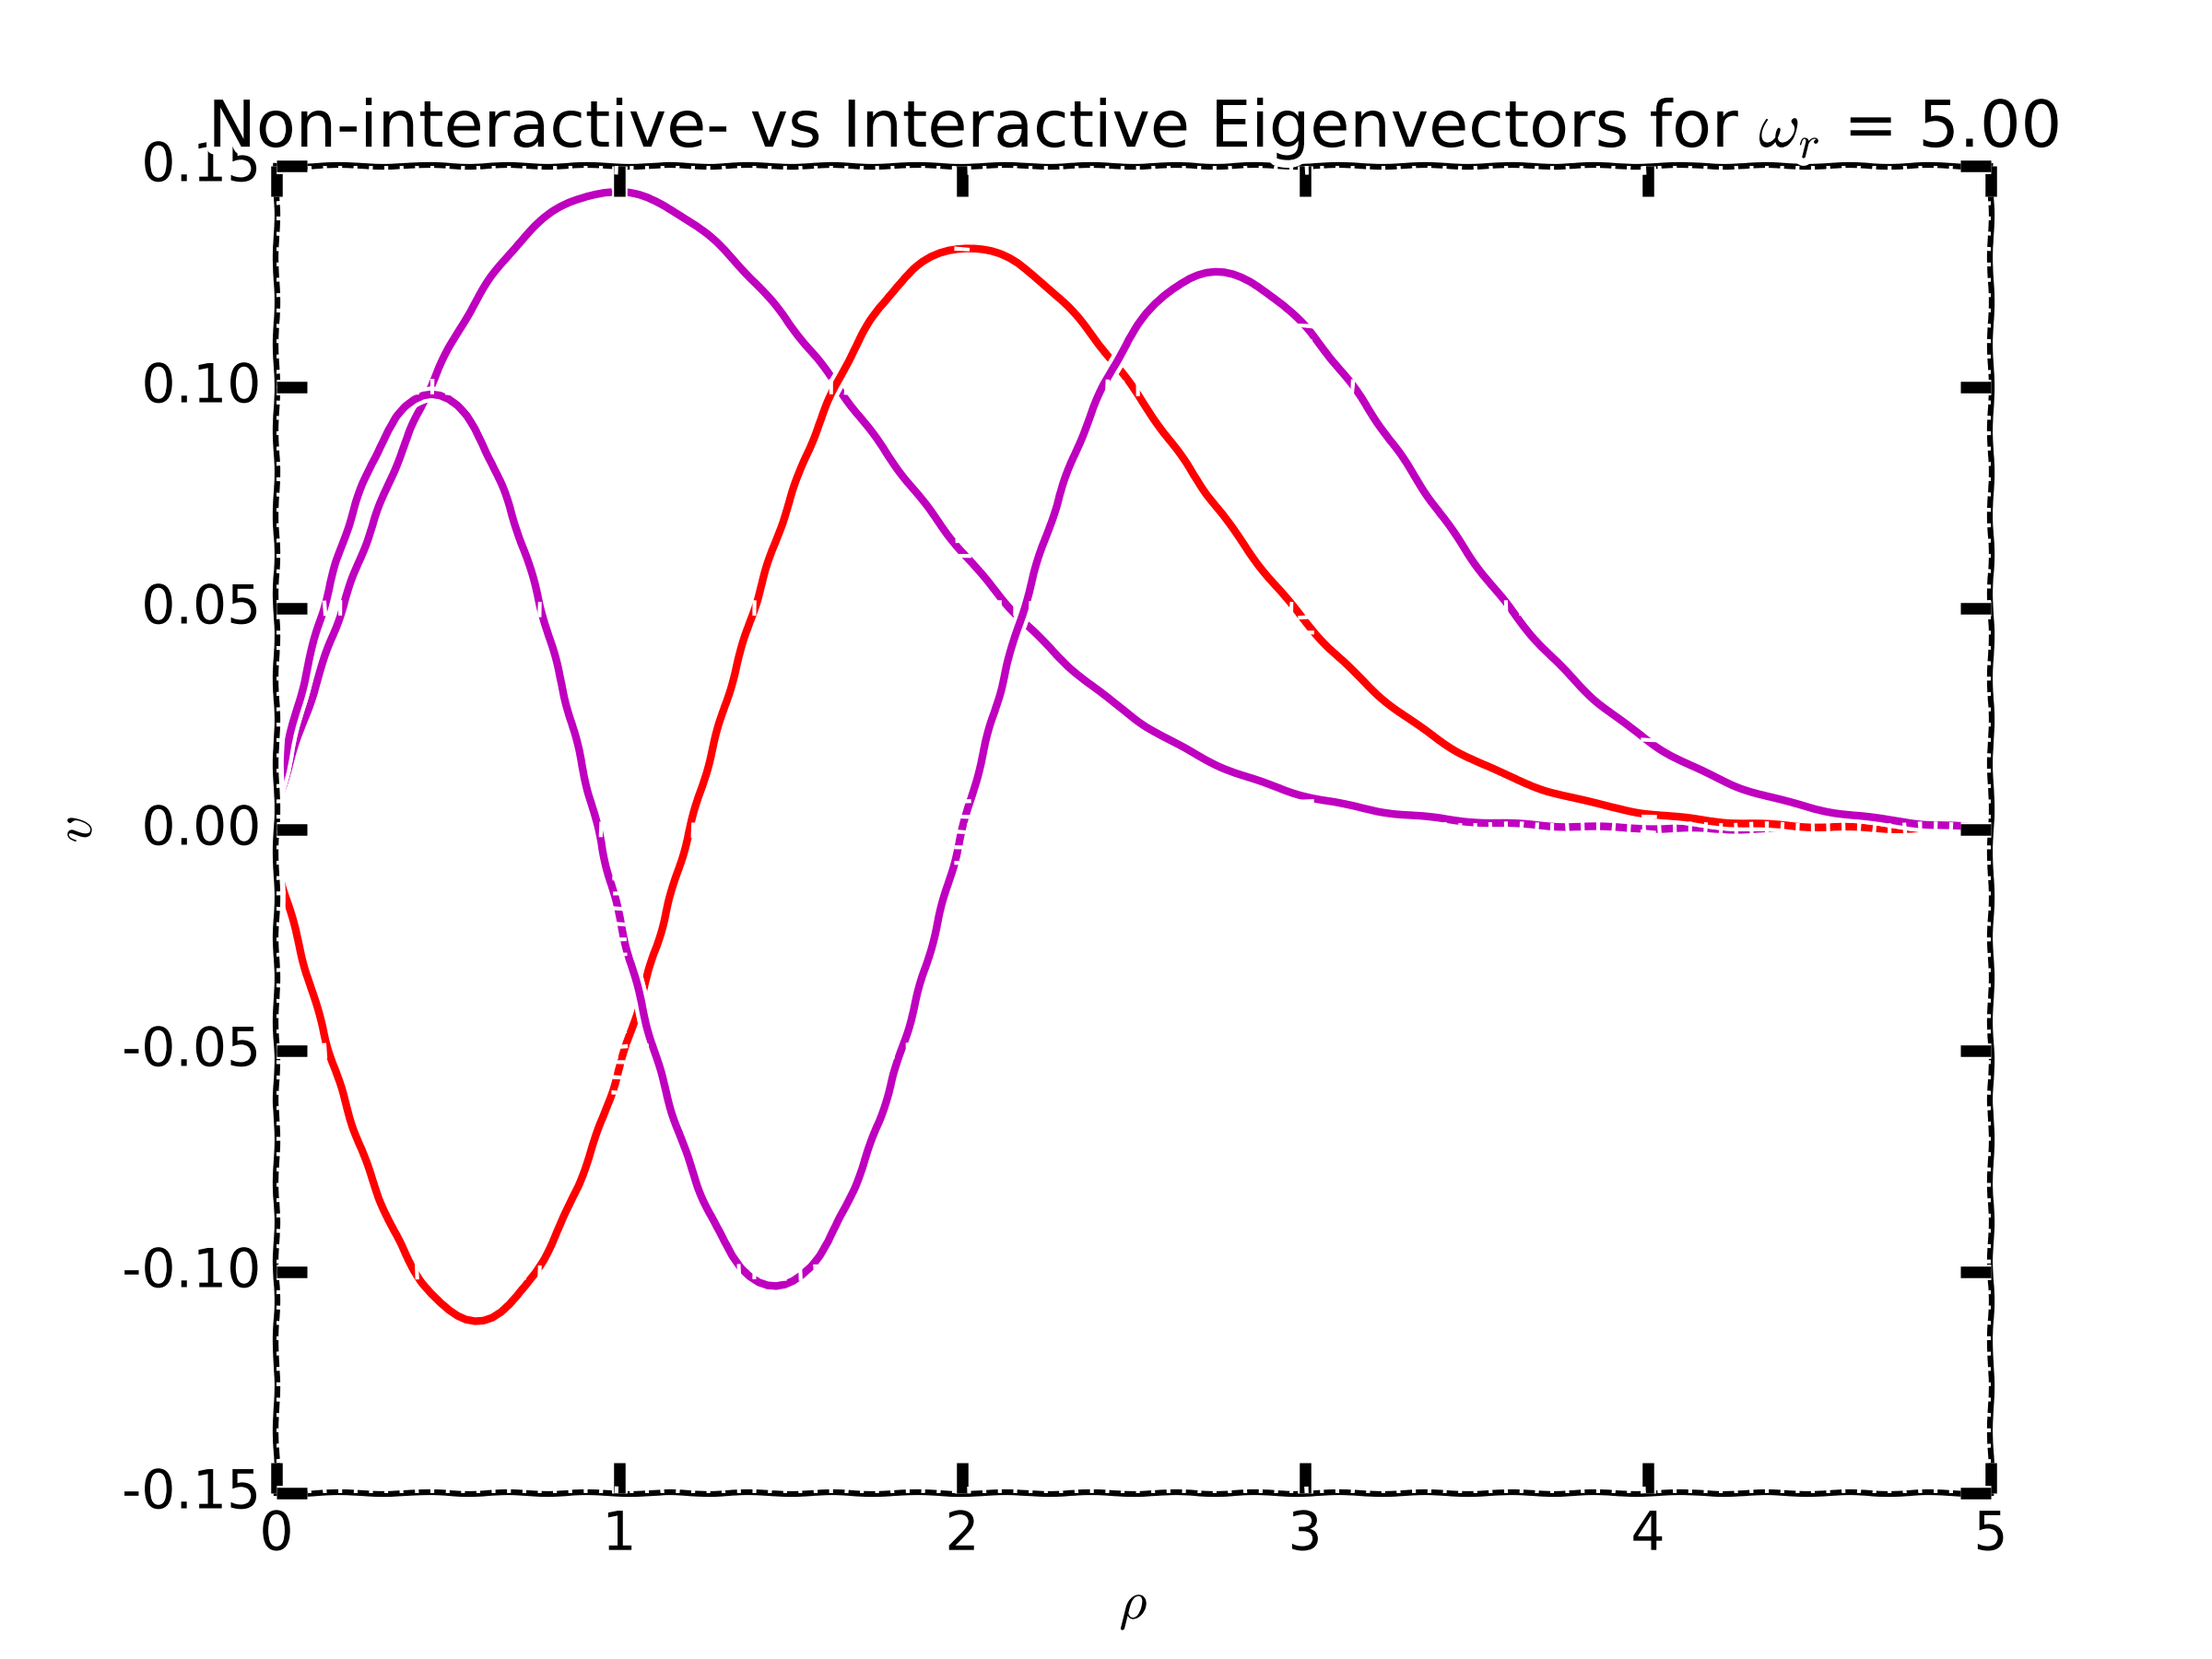
\includegraphics[scale=0.40]{../interacting_eigvecs_at_omega=5000.png}
        \caption{Ground state eigenvectors for both interacting and non-interacting case, at $\omega_r = 5$.}\label{fig:eigvecs-interact5000}
    \end{subfigure}
    \begin{subfigure}[t]{0.45\textwidth}
        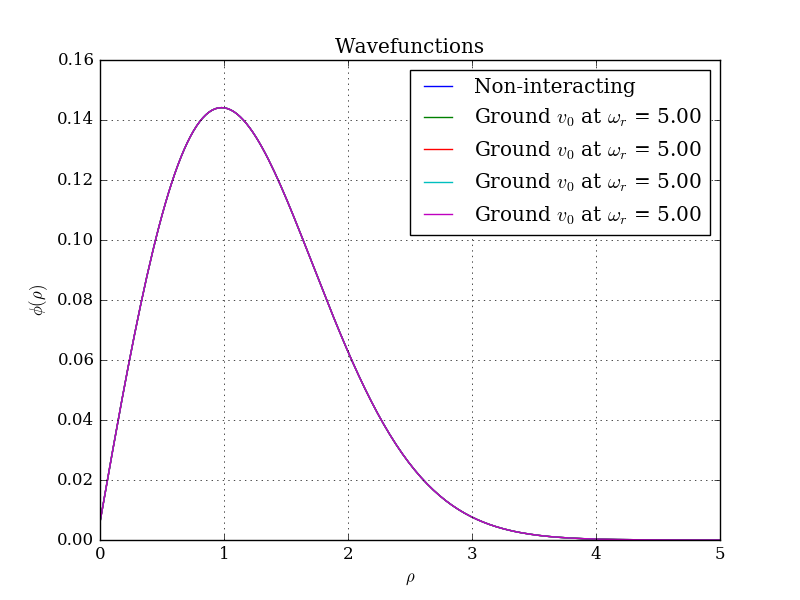
\includegraphics[scale=0.40]{../eigvecs_vs_each_other.png}
        \caption{A non-interacting ground eigenvector, plotted for comparison to ground eigenvectors related to different values of $\omega_r$.}\label{fig:ground-eigvecs-compare}
    \end{subfigure}
    \caption{A set of ground state for interactions at different values of $\omega_r$.}\label{fig:eigvecs-interact}
\end{figure}


\section{Conclusion and discussion}
\section{Appendix - Github} \label{section:github}
\url{https://github.com/theknight1509/FYS4150_Project2}


We got a lot of inspiration from the example-code in \cite[web-site]{example_code}



\begin{thebibliography}{9}
\bibitem{example_code}
  Jensen, M 2016,
  program1.cpp,
  viewed $29^{th}$ September 2016,
  \url{https://github.com/CompPhysics/ComputationalPhysics/blob/master/doc/Programs/LecturePrograms/programs/EigenProblems/cpp/program1.cpp}.
\bibitem{schrodinger_equation}
  Griffiths D.J, 
  Pearson (1995),
  \emph{Introduction to quantum mechanics},
  $2^{nd}$ edition(international).
  
\bibitem{discretize_double_deriv}
	Jensen, M 2016, 
	Computational Physics Lectures: Linear
Algebra methods, 
	viewed $27^{th}$ September 2016, 
	\url{http://compphysics.github.io/ComputationalPhysics/doc/pub/linalg/pdf/linalg-print.pdf} p.12. 

\end{thebibliography}
\end{document}
